\myChapter{G\'en\'eralit\'es sur les PFAS et l'intelligence artificielle}{G\'en\'eralit\'es}
\label{chap:generalites}
\myMiniToc{section}{Sommaire}

\mySection{Introduction}{}
\label{sec:intro-chap1}

La surveillance de la qualit\'e des eaux souterraines est confront\'ee \`a l'\'emergence de contaminants persistants, parmi lesquels les substances per- et polyfluoroalkyl\'ees (PFAS) occupent une place particuli\`ere par leur stabilit\'e chimique, leur mobilit\'e et la diversit\'e de leurs usages.
Dans le m\^eme temps, le d\'eveloppement de l'\textbf{intelligence artificielle} et de l'\textbf{apprentissage automatique} (\emph{machine learning}, ML) fournit des outils puissants pour analyser des volumes importants de donn\'ees environnementales, combiner des sources d'information h\'et\'erog\`enes et appuyer la prise de d\'ecision.
Ce premier chapitre a pour objectif de r\'eunir les \textbf{notions fondamentales} qui seront mobilis\'ees dans la suite du m\'emoire.
Nous y pr\'esentons d'abord le contexte des PFAS : d\'efinition, propri\'et\'es physicochimiques, principaux usages, sources de contamination, devenir environnemental, enjeux de surveillance des eaux souterraines et cadre r\'eglementaire (section~\ref{sec:pfas}).
Nous introduisons ensuite les paradigmes de l'apprentissage automatique, le bagging, le boosting et le stacking (section~\ref{sec:ml-ensemble}), puis les \textbf{graphes} et les r\'eseaux de neurones sur graphes, en particulier les graphes h\'et\'erog\`enes et le Transformeur de Graphe h\'et\'erog\`enes (section~\ref{sec:graphes-gnn}).
Enfin, nous pr\'esentons les principaux outils d'\textbf{interpr\'etabilit\'e} des mod\`eles, avec un accent sur l'approche SHAP (section~\ref{sec:interpretabilite}), afin de pr\'eparer l'analyse des r\'esultats qui sera men\'ee dans les chapitres suivants.



\mySection{Substances per- et polyfluoroalkyl\'ees (PFAS)}{}
\label{sec:pfas}

Les PFAS occupent une place \`a part parmi les contaminants de l'eau : leur persistance, leur mobilit\'e et le nombre tr\`es \'elev\'e de compos\'es potentiels compliquent la surveillance classique.
Cette section en pr\'esente la \textbf{d\'efinition}, les \textbf{propri\'et\'es physicochimiques}, les \textbf{usages} \`a l'origine des rejets, le \textbf{devenir} dans l'environnement (sources et transport), les enjeux de \textbf{surveillance des eaux souterraines}, puis les \textbf{risques sanitaires} et le \textbf{cadre r\'eglementaire}.


\mySubSection{D\'efinition et propri\'et\'es physicochimiques}{}
\label{sec:pfas-proprietes}

\mySubSubSection{Une famille chimique vaste et h\'et\'erog\`ene}{}

Les \textbf{substances per- et polyfluoroalkyl\'ees} (PFAS, \emph{per- and polyfluoroalkyl substances}) d\'esignent une famille de compos\'es organiques de synth\`ese dont le nombre exact d\'epasse largement quelques centaines de mol\'ecules : les inventaires r\'eglementaires et scientifiques recensent de l'ordre de \textbf{4\,000 \`a plus de 10\,000} structures selon les crit\`eres d'inclusion retenus~\cite{gluge2020pfas}.
Toutes partagent l'id\'ee d'une cha\^ine carbon\'ee aliphatique dont une partie des atomes d'hydrog\`ene est remplac\'ee par du \textbf{fluor}.

Historiquement, une d\'efinition de r\'ef\'erence exigeait la pr\'esence d'un groupement \textbf{perfluoroalkyl\'e} satur\'e en fluor.
L'Organisation de coop\'eration et de d\'eveloppement \'economiques (OCDE) a ensuite \'elargi le champ \`a toute substance contenant au moins un groupement m\'ethyl\`ene ou m\'ethyle \textbf{enti\`erement fluor\'e}, afin d'int\'egrer des mol\'ecules utilis\'ees dans des fili\`eres r\'ecentes (semi-conducteurs, batteries, mat\'eriaux haute performance).
Le terme \textbf{PFAS} fonctionne ainsi comme un \textbf{parapluie r\'eglementaire et analytique}, et non comme le nom d'un produit unique.


\mySubSubSection{La liaison carbone--fluor et la persistance}{}

La liaison \textbf{carbone--fluor} (C--F) est l'une des plus fortes de la chimie organique (de l'ordre de 485~kJ/mol).
Elle conf\`ere aux mol\'ecules une inertie remarquable face \`a la chaleur, aux oxydants et aux enzymes microbiennes.
C'est ce qui justifie le surnom de \emph{polluants \'eternels} : contrairement \`a de nombreux hydrocarbures, les PFAS ne sont pas facilement \textbf{biod\'egrad\'es} dans les conditions naturelles~\cite{prevedouros2006pfas}.
Leur pr\'esence dans les sols, les eaux et certains biotes peut donc se prolonger \textbf{d\'ecennies} apr\`es l'arr\^et des \'emissions \`a la source.

On oppose en pratique :
\begin{itemize}
    \item les compos\'es \textbf{perfluoroalkyl\'es} : la cha\^ine est satur\'ee en fluor (hors groupe fonctionnel) ;
    \item les compos\'es \textbf{polyfluoroalkyl\'es} : la fluorination est partielle ; ils peuvent se transformer en d\'eriv\'es plus persistants, appel\'es \textbf{pr\'ecurseurs}.
\end{itemize}

Les compos\'es historiques \`a \textbf{cha\^ine longue} (souvent $\geq$ 6--8 atomes de carbone pour les PFCA) comme le PFOA ou le PFOS ont \'et\'e massivement produits \`a partir des ann\'ees 1950.
Sous pression r\'eglementaire, l'industrie s'est orient\'ee vers des \textbf{cha\^ines courtes} (C4--C6), pr\'esent\'ees comme des alternatives ; celles-ci restent toutefois mobiles et persistantes dans l'environnement.


\mySubSubSection{Groupes fonctionnels, tensioactivit\'e et r\'etention dans les sols}{}

Selon le \textbf{groupe fonctionnel} terminal, on classe notamment :
\begin{itemize}
    \item les \textbf{acides perfluorocarboxyliques} (PFCA), par exemple l'acide perfluorooctano\"ique (PFOA) ;
    \item les \textbf{acides perfluoroalkylsulfoniques} (PFSA), par exemple le sulfonate de perfluorooctane (PFOS).
\end{itemize}
Le tableau~\ref{tab:classes-pfas} illustre d'autres familles courantes.

\begin{table}[h!]
    \centering
    \caption{Principales classes de PFAS et propri\'et\'es associ\'ees (synth\`ese p\'edagogique).}
    \label{tab:classes-pfas}
    \begin{tabular}{lllp{4.2cm}}
        \hline
        Classe & Groupe & Exemple & Propri\'et\'e dominante \\
        \hline
        PFCA & Carboxylate & PFOA (C8) & Persistance, adsorption, bioaccumulation \\
        PFSA & Sulfonate & PFOS (C8) & Tensioactivit\'e, bioaccumulation, stabilit\'e \\
        Fluorot\'elom\`eres & Alcools, sulfonates & 6:2 FTS & Pr\'ecurseur de PFCA \\
        PFPE & \'Ether perfluor\'e & Lubrifiants & R\'esistance thermique \\
        \hline
    \end{tabular}
\end{table}

Les PFAS sont \textbf{amphiphiles} : une cha\^ine fluor\'ee hydrophobe et lipophobe est reli\'ee \`a une t\^ete polaire hydrophile.
Cette structure explique leur efficacit\'e comme \textbf{tensioactifs} (r\'eduction de la tension superficielle), notamment dans les mousses anti-incendie, et leur tendance \`a s'accumuler aux \textbf{interfaces} air--eau et solide--eau en zone non satur\'ee~\cite{brusseau2019pfas}.

La figure~\ref{fig:pfos-structure} illustre la structure d'un PFAS non polym\'erique, le sulfonate de perfluorooctane (PFOS).

\begin{figure}[H]
    \centering
    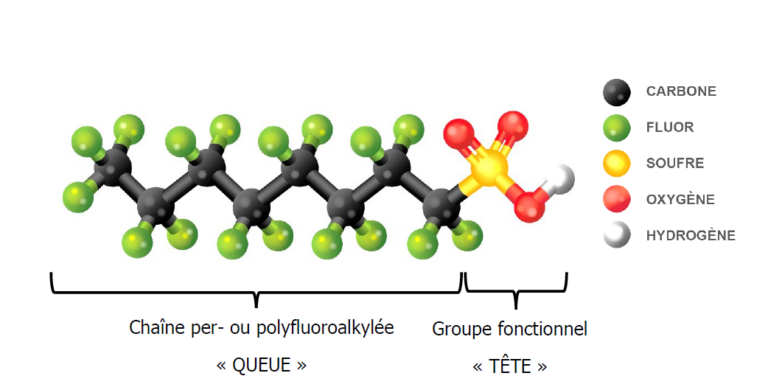
\includegraphics[width=0.82\linewidth]{Chap1/images/repre_pfas_polyflore.png}
    \caption{Repr\'esentation sch\'ematique du PFOS (acide perfluorooctanesulfonique, C$_8$F$_{17}$SO$_3$H ou C$_8$F$_{17}$SO$_3^-$). Source : adapt\'e de~\cite{vds2025pfas}.}
    \label{fig:pfos-structure}
\end{figure}
La structure illustr\'ee met en \'evidence la dualit\'e de la cha\^ine perfluor\'ee (queue) et du groupe sulfonate (t\^ete polaire), qui fonde \`a la fois la persistance et la tensioactivit\'e du compos\'e.

La \textbf{longueur de cha\^ine} modifie la solubilit\'e, la mobilit\'e et la bioaccumulation : les cha\^ines courtes se d\'eplacent plus facilement dans l'eau ; les cha\^ines longues sont davantage retenues par les mati\`eres organiques du sol et les prot\'eines.


\mySubSection{Usages, sources et devenir environnemental}{}
\label{sec:pfas-usages-sources}
\label{sec:pfas-usages}
\label{sec:pfas-transport}

La pr\'esence des PFAS dans l'environnement d\'ecoule d'une cha\^ine causale continue : des choix industriels engendrent des rejets, qui alimentent des sources de contamination, lesquelles propagent les compos\'es vers les milieux r\'ecepteurs selon des m\'ecanismes physiques bien document\'es.
Cette sous-section d\'etaille successivement les usages \`a l'origine des \'emissions, la nature des sources, les voies de dispersion, et le mod\`ele conceptuel source-voie-r\'ecepteur qui en synth\'etise la logique.


\mySubSubSection{Usages industriels}{}

Les PFAS ne sont pas des polluants accidentels ponctuels : ils r\'esultent de \textbf{choix industriels} r\'ep\'et\'es sur plus de soixante ans.
Leur combinaison de r\'epellence (eau, graisses), de stabilit\'e thermique et de faible friction a conduit \`a de nombreuses applications~\cite{gluge2020pfas} :
\begin{itemize}
    \item \textbf{Textiles et habillement} : imperm\'eabilit\'e, r\'esistance aux taches ;
    \item \textbf{Emballages alimentaires} et papier trait\'e : barri\`ere \`a l'huile et \`a l'eau ;
    \item \textbf{Mousses anti-incendie} pour feux d'hydrocarbures (films aqueux AFFF) ;
    \item \textbf{Industrie chimique et \'electronique} : fluides de proc\'ed\'e, lubrifiants, rev\^etements ;
    \item \textbf{Cosm\'etiques et produits d'entretien} : certains compos\'es sont aujourd'hui progressivement interdits ou restreints selon les juridictions.
\end{itemize}

\`A chaque \textbf{cycle de vie} (fabrication, utilisation, traitement des d\'echets), une fraction des PFAS peut \^etre rejet\'ee dans l'air, l'eau ou les sols.
Les proc\'ed\'es de traitement classiques des eaux us\'ees ou des lixiviats de d\'echarges ne sont g\'en\'eralement pas con\c{c}us pour \textbf{casser} la liaison C--F : une partie des compos\'es traverse les stations et retourne vers les milieux naturels~\cite{hu2016pfas,prevedouros2006pfas}.


\mySubSubSection{Typologie des sources de contamination}{}

On classe couramment les sources selon leur intensit\'e et leur localisation :
\begin{enumerate}
    \item \textbf{Sources ponctuelles industrielles} : usines de synth\`ese ou de transformation de produits fluor\'es, rejets historiques stock\'es dans les sols ;
    \item \textbf{Sites militaires et a\'eroportuaires} : entra\^inements au feu avec mousses AFFF, souvent identifi\'es comme \textbf{hotspots} de contamination des nappes ;
    \item \textbf{Sources diffuses} : stations d'\'epuration, sites d'enfouissement, ruissellement urbain transportant des r\'esidus de produits de consommation.
\end{enumerate}

Des \'etudes \`a l'\'echelle r\'egionale ont montr\'e une association statistique entre la pr\'esence de PFAS dans l'eau potable et la proximit\'e d'installations industrielles, de bases militaires ou de stations d'\'epuration~\cite{hu2016pfas}.
La mousse \textbf{AFFF} m\'erite une attention particuli\`ere : d\'evelopp\'ee pour \'eteindre les feux de carburant, elle a \'et\'e d\'eploy\'ee \`a grande \'echelle sur les a\'erodromes et casernes ; les m\'elanges infiltr\'es dans le sol peuvent alimenter des panaches souterrains durables.


\mySubSubSection{M\'ecanismes de transport dans l'air, le sol et l'eau}{}

Une fois rejet\'es, les PFAS suivent des trajectoires \textbf{coupl\'ees} :
\begin{itemize}
    \item \textbf{Eaux souterraines} : transport principalement \textbf{advectif} avec le flux de la nappe ; la vitesse d\'epend de la conductivit\'e hydraulique, de la porosit\'e, du gradient hydraulique et du degr\'e de r\'etention sur les sols (mati\`ere organique, min\'eraux)~\cite{brusseau2019pfas}.
    \item \textbf{Zone vadose} (non satur\'ee) : accumulation possible aux interfaces air--eau, formant un \textbf{r\'eservoir} lib\'er\'e progressivement lors des pluies ;
    \item \textbf{Atmosph\`ere} : certains pr\'ecurseurs volatils (fluorot\'elom\`eres) peuvent \^etre transport\'es sur de longues distances avant d\'ep\^ot sec ou humide, contribuant \`a une contamination \textbf{ubiquitaire} m\^eme loin des sites industriels~\cite{guelfo2021pfas}.
\end{itemize}

Sur des aquif\`eres perm\'eables \`a faible teneur en carbone, des panaches de plusieurs \textbf{kilom\`etres} ont \'et\'e d\'ecrits en aval de sources ponctuelles.
Le comportement ne se r\'eduit donc pas \`a une dilution imm\'ediate : la persistance et la mobilit\'e conjointes expliquent l'\'etendue spatiale des probl\`emes.


\mySubSubSection{Le sch\'ema source, voie et r\'ecepteur}{}
\label{sec:pfas-svr}

En \'evaluation des risques environnementaux, le devenir des PFAS est souvent repr\'esent\'e par le mod\`ele \textbf{source, voie et r\'ecepteur}~\cite{brusseau2019pfas,guelfo2021pfas} :
\begin{itemize}
    \item \textbf{Source} : activit\'e humaine qui \'emet les PFAS (usine, base militaire, rejet urbain) ;
    \item \textbf{Voie} : milieu qui transporte le polluant (sol, eau souterraine, eau de surface, air) ;
    \item \textbf{R\'ecepteur} : milieu ou organisme expos\'e (nappe exploit\'ee, puits, rivi\`ere, population).
\end{itemize}

Ce sch\'ema aide \`a structurer la pens\'ee, ind\'ependamment des outils math\'ematiques utilis\'es ensuite pour l'analyse des donn\'ees.
La figure~\ref{fig:voies-contamination-pfas} en illustre la d\'eclinaison concr\`ete pour les PFAS.

\begin{figure}[htbp]
    \centering
    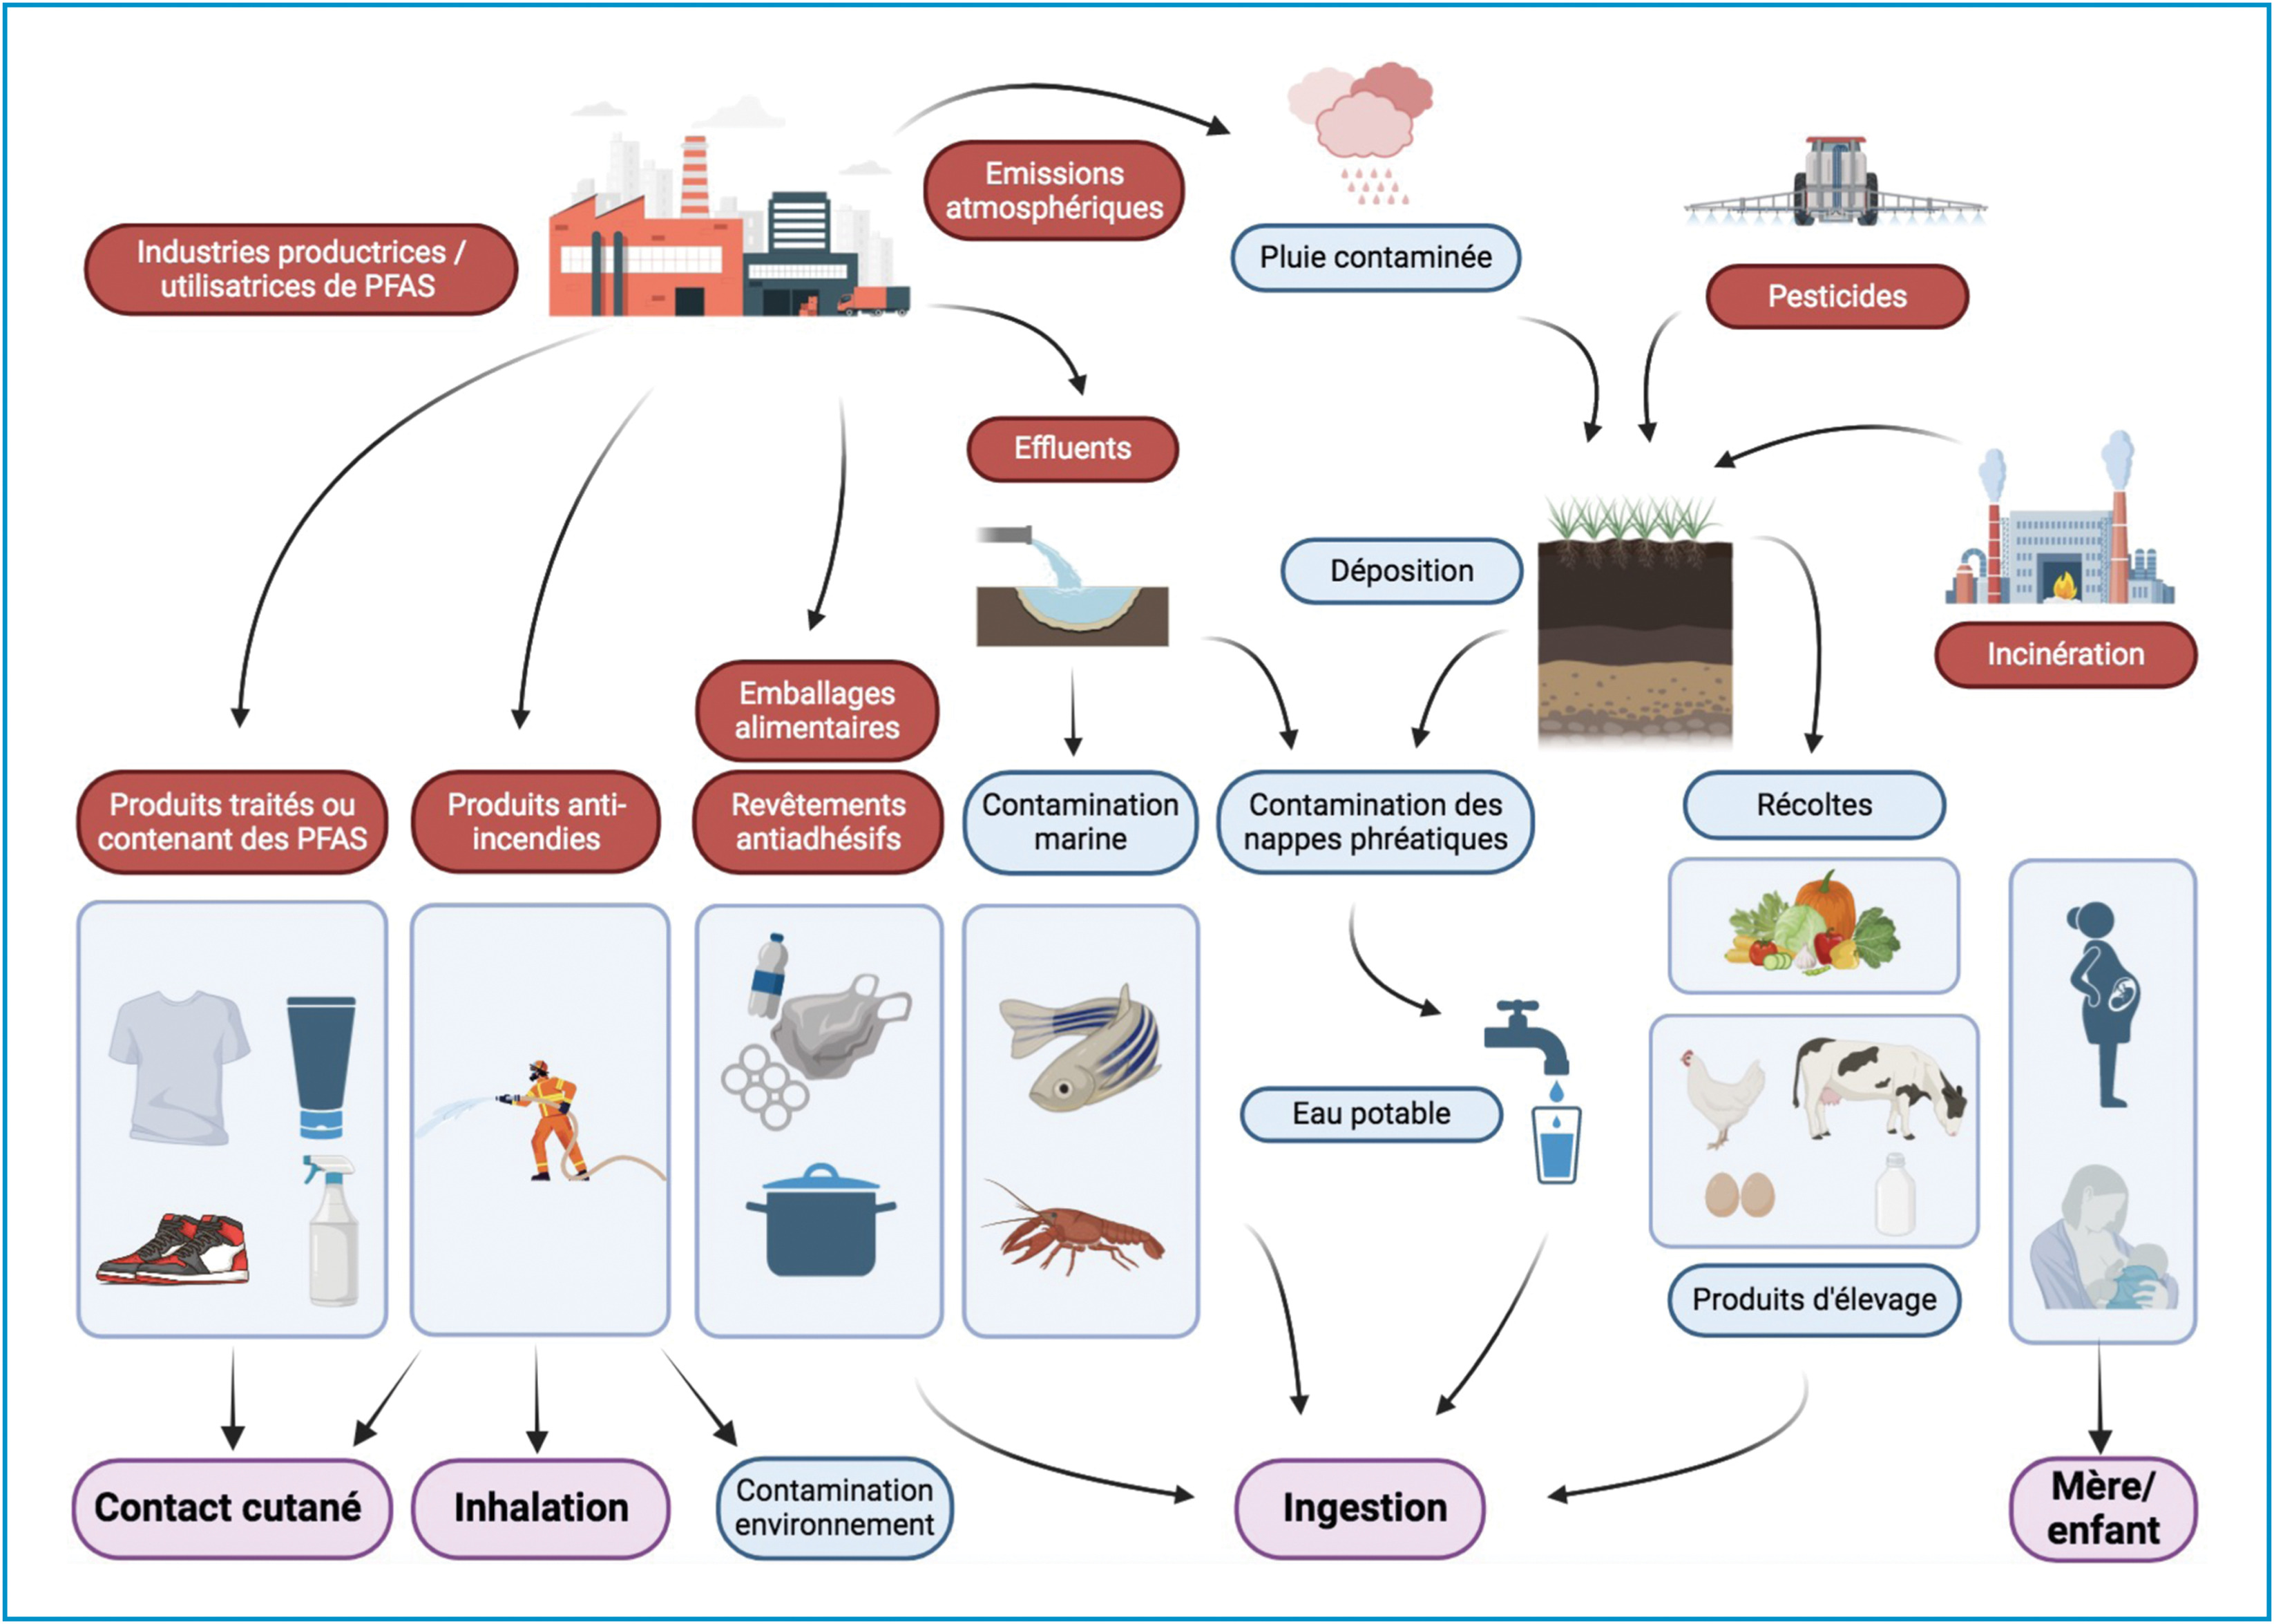
\includegraphics[width=0.92\linewidth]{Chap1/images/voie_contamination_pfas.jpg}
    \caption{Voies possibles de contamination humaine aux PFAS (sources directes en rouge, contamination indirecte via sol ou eau en bleu, voies d'exposition en violet). Source : adapt\'e de~\cite{fct2024pfasfigures}.}
    \label{fig:voies-contamination-pfas}
\end{figure}

La figure met en \'evidence que les rejets industriels ou l'usage de produits de consommation alimentent d'abord les milieux (sol, eau), avant d'atteindre l'homme par l'eau potable, l'alimentation ou d'autres voies d'exposition.
On observe par ailleurs une \textbf{co-occurrence} fr\'equente avec d'autres polluants organiques sur les m\^emes sites : solvants chlor\'es (TCE, PCE), hydrocarbures, additifs (MTBE).
Ces co-contaminants partagent souvent une histoire industrielle commune, m\^eme si leurs propri\'et\'es de transport diff\`erent.


\mySubSection{Surveillance des eaux souterraines et limites de la mesure}{}
\label{sec:pfas-surveillance}

Les \textbf{eaux souterraines} constituent un enjeu majeur car elles alimentent une part importante de l'eau potable et de l'irrigation.
Les PFAS y sont d'autant plus pr\'eoccupants qu'ils peuvent migrer \textbf{loin} de la source visible et demeurer longtemps \`a des concentrations tr\`es faibles mais significatives sur le plan sanitaire~\cite{hu2016pfas}.

La \textbf{surveillance} repose classiquement sur :
\begin{itemize}
    \item le pr\'el\`evement sur des \textbf{puits} ou points de contr\^ole ;
    \item l'analyse en laboratoire par chromatographie de type LC-MS/MS, ciblant un \textbf{panier} de compos\'es (souvent quelques dizaines de mol\'ecules parmi des milliers possibles) ;
    \item la comparaison aux \textbf{seuils r\'eglementaires} ou aux valeurs guides sanitaires.
\end{itemize}

Plusieurs limites structurelles expliquent la difficult\'e d'un suivi exhaustif :
\begin{itemize}
    \item \textbf{Co\^ut} \'elev\'e d'une analyse multi-compos\'es ;
    \item \textbf{Couverture spatiale} incompl\`ete (impossible de mesurer tous les puits d'une r\'egion) ;
    \item \textbf{Non-d\'etection} fr\'equente : une valeur nulle ne signifie pas toujours l'absence de PFAS, mais parfois une concentration sous le seuil de d\'etection de la m\'ethode~\cite{guelfo2021pfas} ;
    \item \textbf{H\'et\'erog\'en\'eit\'e} des protocoles entre r\'egions et campagnes.
\end{itemize}

Ces contraintes expliquent l'int\'er\^et, dans la litt\'erature r\'ecente, pour des approches de \textbf{priorisation} fond\'ees sur des donn\'ees d\'ej\`a disponibles (contexte g\'eologique, proximit\'e d'activit\'es, qualit\'e de l'eau)~\cite{dong2024pfas}.


\mySubSection{Impacts sanitaires et cadre r\'eglementaire}{}
\label{sec:pfas-reglementation}

\mySubSubSection{Voies d'exposition et effets document\'es}{}

L'exposition humaine aux PFAS peut intervenir par plusieurs \textbf{voies}~\cite{sunderland2019pfas} :
\begin{itemize}
    \item \textbf{Eau potable} contamin\'ee (voie souvent dominante pr\`es des sites pollu\'es) ;
    \item \textbf{Alimentation} (poissons d'eau douce, produits d'origine animale bioaccumulants) ;
    \item \textbf{Poussi\`eres int\'erieures} et produits de consommation trait\'es ;
    \item \textbf{Contact professionnel} sur les sites de production ou d'usage intensif.
\end{itemize}

Les effets sanitaires \'etudi\'es \`a des doses environnementales tr\`es basses (ng/L dans l'eau) incluent notamment :
\begin{itemize}
    \item des effets sur le \textbf{syst\`eme immunitaire} (r\'eponse vaccinale);
    \item des perturbations \textbf{thyro\"idiennes} et m\'etaboliques (lipides);
    \item des impacts sur le \textbf{d\'eveloppement f\oe tal} (poids \`a la naissance, pr\'e\'eclampsie);
    \item pour certains compos\'es, des associations avec des \textbf{cancers} (rein, testicules) dans les cohortes les plus expos\'ees.
\end{itemize}

La figure~\ref{fig:pfas-pathologies} synth\'etise les pathologies suspect\'ees d'\^etre li\'ees \`a la toxicit\'e des PFAS chez l'humain.

\begin{figure}[H]
    \centering
    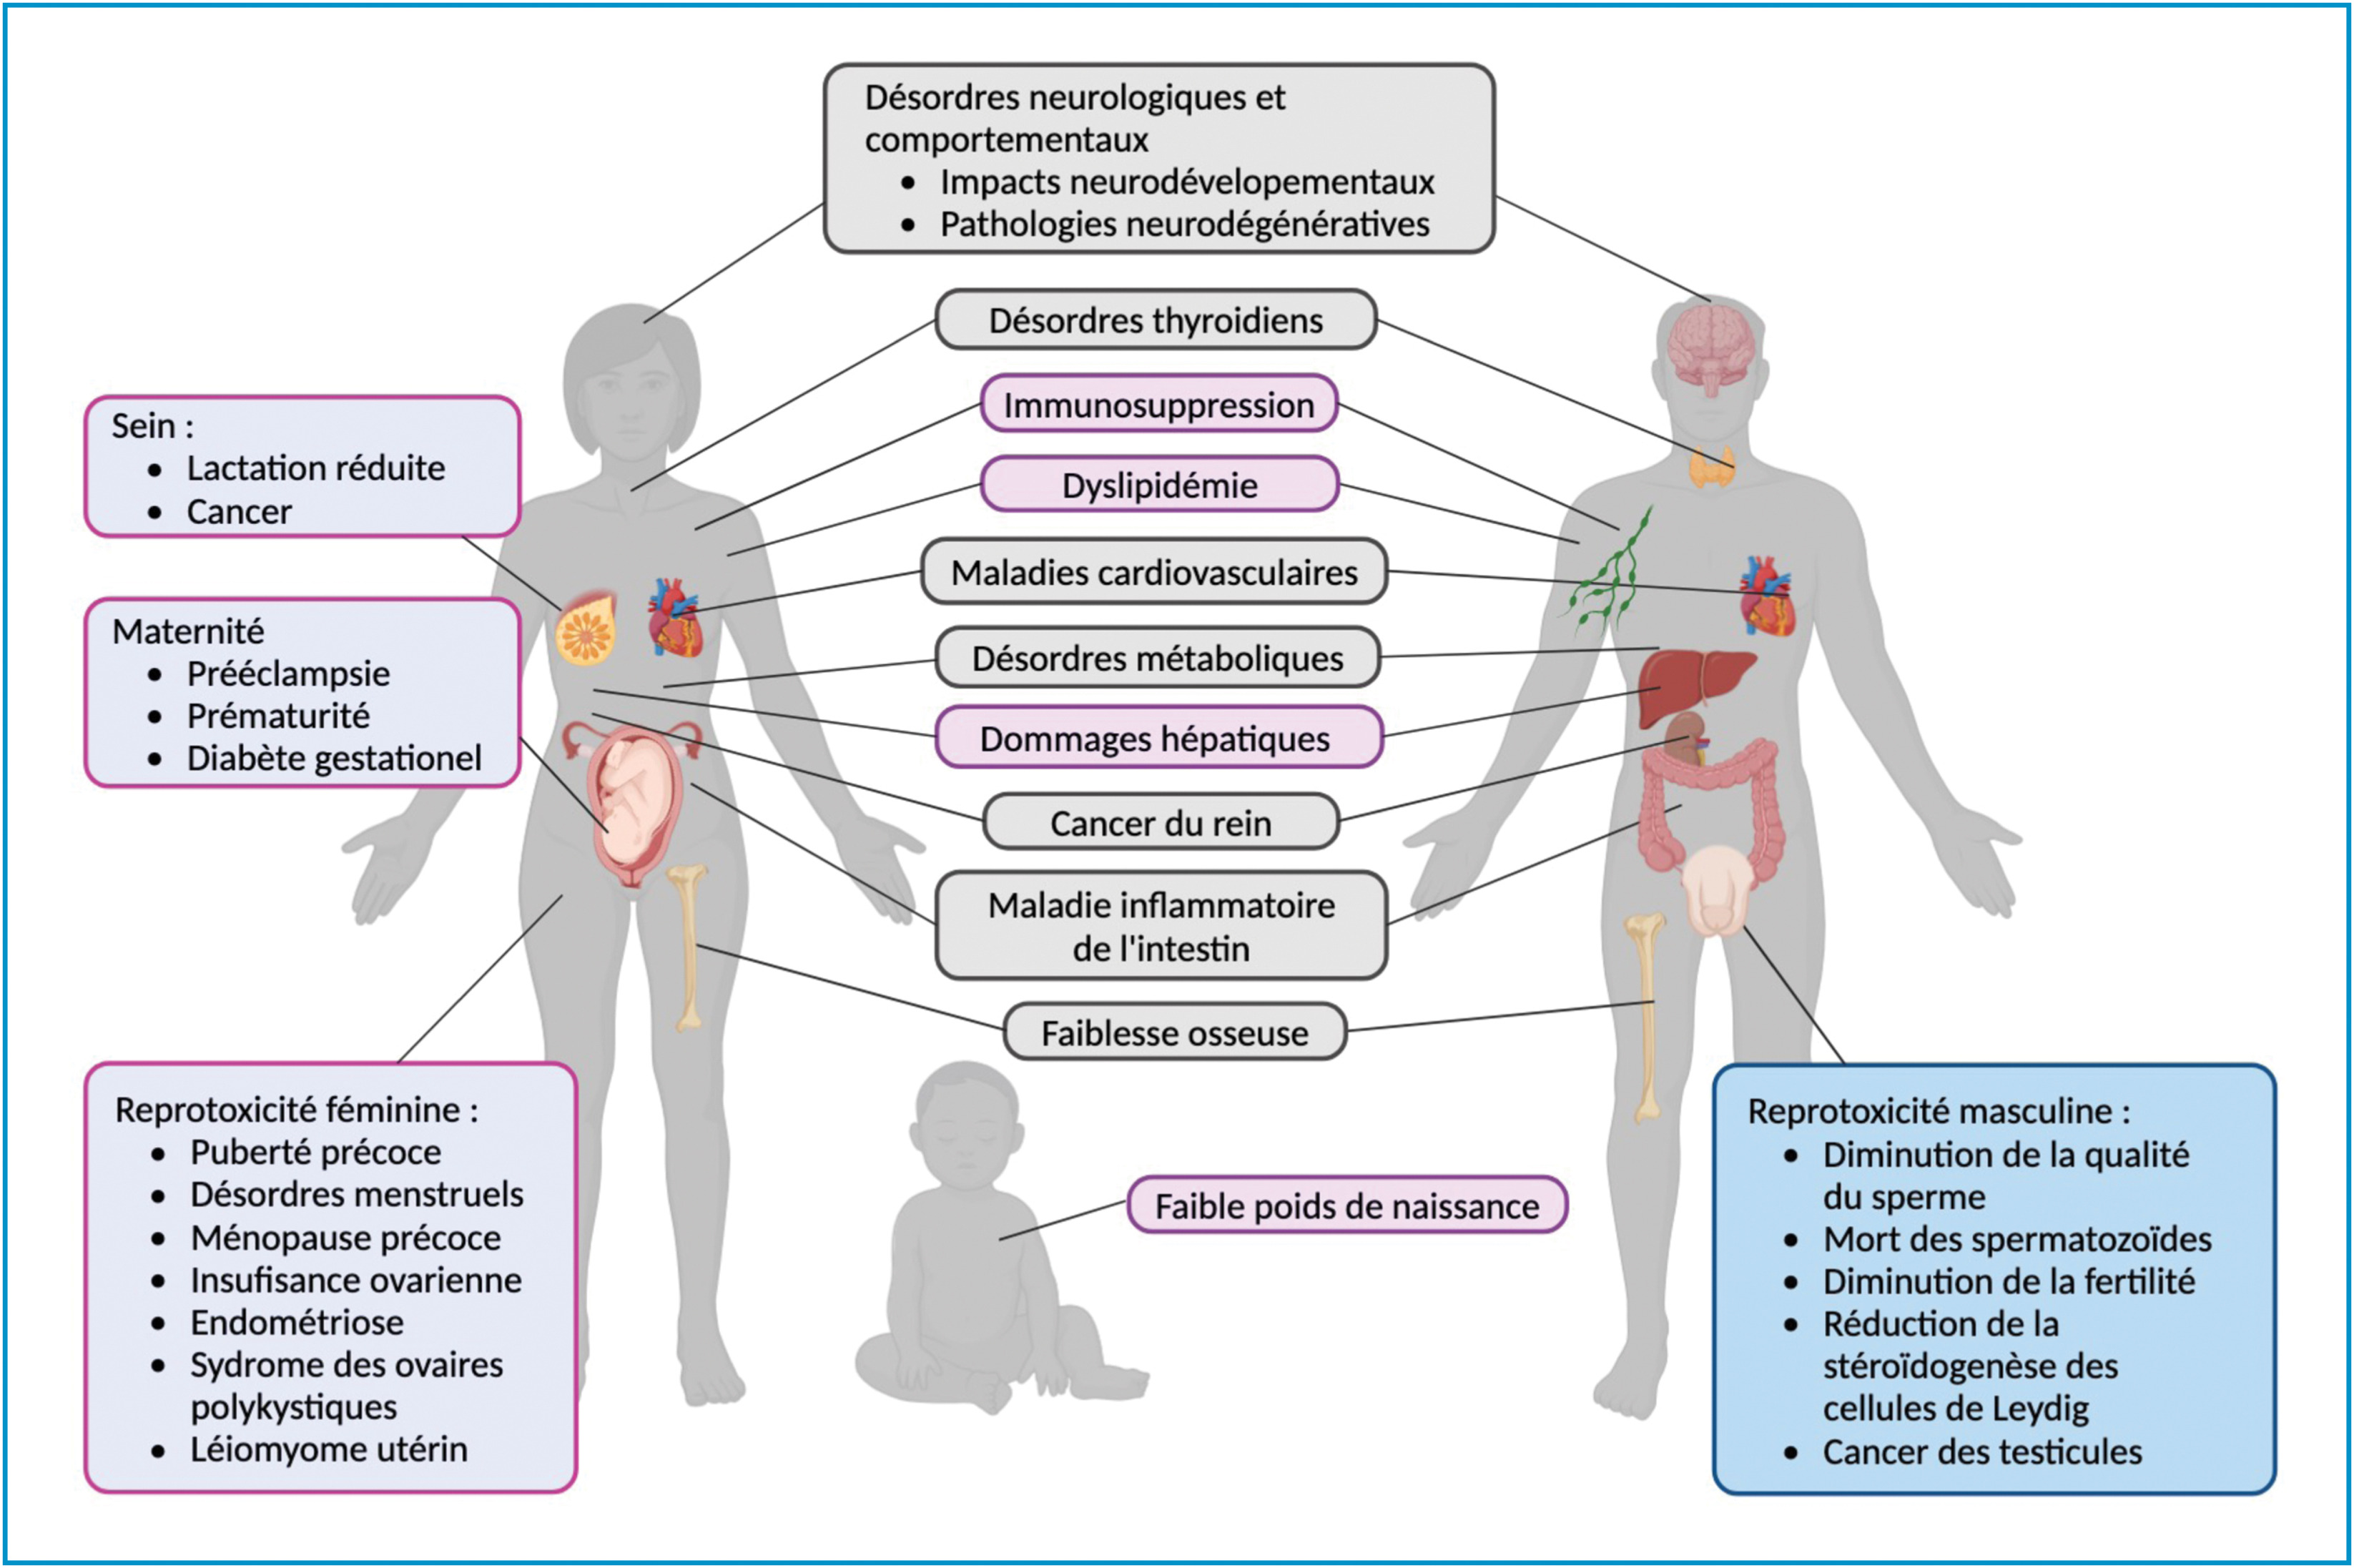
\includegraphics[width=0.88\linewidth]{Chap1/images/human_pfas_pathologies.jpg}
    \caption{Pathologies suspect\'ees d'\^etre induites par la toxicit\'e des PFAS (effets \'epid\'emiologiques corrobor\'es au centre ; autres effets document\'es en gris ; effets reprotoxiques sur les c\^ot\'es). Source : adapt\'e de~\cite{fct2024pfasfigures}.}
    \label{fig:pfas-pathologies}
\end{figure}
Cette synth\`ese illustre que plusieurs organes et fonctions (immunit\'e, thyro\"ide, d\'eveloppement f\oe tal, reproduction) figurent parmi les effets les plus document\'es, justifiant le renforcement des seuils r\'eglementaires et des programmes de surveillance.

Le tableau~\ref{tab:pfas-sante} en donne une vue synth\'etique tabulaire ; il ne remplace pas une analyse toxicologique d\'etaill\'ee.

\begin{table}[h!]
    \centering
    \caption{Exemples d'effets sanitaires associ\'es \`a l'exposition aux PFAS (synth\`ese).}
    \label{tab:pfas-sante}
    \begin{tabular}{lp{5.5cm}p{4cm}}
        \hline
        Syst\`eme & Effets document\'es & Populations sensibles \\
        \hline
        Immunitaire & Diminution de la r\'eponse vaccinale & Enfants \\
        Endocrinien & Perturbation thyro\"idienne, lipides & Adultes \\
        D\'eveloppement & Faible poids \`a la naissance & Femmes enceintes \\
        Reproduction & Fertilit\'e, complications gestationnelles & Adultes \\
        Canc\'er (certains compos\'es) & Rein, testicules (associations) & Expos\'es professionnels \\
        \hline
    \end{tabular}
\end{table}


\mySubSubSection{\'Evolution du cadre r\'eglementaire}{}

Face \`a ces risques, les seuils admissibles ont fortement baiss\'e au cours des derni\`eres ann\'ees.
Aux \'Etats-Unis, l'EPA a publi\'e en 2016 un \textbf{avis sanitaire} (\emph{health advisory}) \`a \textbf{70~ng/L} pour la somme PFOA+PFOS~\cite{epa2016pfas}, puis en 2024 un \textbf{r\`eglement national} sur l'eau potable fixant des limites maximales de contaminants (MCL) \`a \textbf{4~ng/L} pour le PFOA et le PFOS \textbf{s\'epar\'ement}~\cite{epa2023npdwr}.
Cette dualit\'e (avis historique vs limites r\'ecentes plus strictes) illustre la \textbf{rapidit\'e} de l'\'evolution normative.

En Europe, la directive sur l'eau potable (2020/2184/UE) encadre un sous-ensemble de PFAS :
\begin{itemize}
    \item une limite sur la \textbf{somme de 20 PFAS} prioritaires (indicateur \texttt{PFAS Total}, valeur param\'etrique de l'ordre de 0,1~$\mu$g/L) ;
    \item une limite sur le \textbf{total des PFAS} mesur\'es au-del\`a d'un seuil de quantification (indicateur \texttt{PFAS TQS}, de l'ordre de 0,5~$\mu$g/L).
\end{itemize}

Des initiatives nationales compl\`etent ce cadre (programmes de surveillance en Allemagne, Pays-Bas, Danemark, etc.).
En France, des textes r\'ecents visent \`a restreindre certains usages non essentiels (cosm\'etiques, textiles, produits de loisirs) et \`a renforcer la fiscalit\'e ou la redevance sur les rejets industriels, dans une logique de \textbf{pr\'evention} \`a la source.

Quelle que soit la juridiction, le message commun est le suivant : les concentrations d'int\'er\^et sont \textbf{tr\`es faibles}, la liste des compos\'es \`a suivre \textbf{change}, et la surveillance doit \^etre \textbf{\'etendue} dans le temps et dans l'espace, ce qui pose un d\'efi logistique consid\'erable pour les gestionnaires de l'eau.

Sur le continent africain, les r\'eglementations nationales sp\'ecifiques aux PFAS font encore largement d\'efaut.
Les lignes directrices de l'Organisation mondiale de la sant\'e pour la qualit\'e de l'eau potable~\cite{who2022drinking} constituent, dans ce contexte, la r\'ef\'erence disponible pour les pays d'Afrique subsaharienne.
Au Cameroun en particulier, aucune norme nationale d\'edi\'ee aux PFAS n'est actuellement en vigueur ; la surveillance s'appuie sur des valeurs guides internationales, rendant d'autant plus pertinentes les approches fond\'ees sur des donn\'ees contextuelles disponibles pour estimer le risque sans analyse cibl\'ee syst\'ematique.

L'ensemble de ces contraintes (analytiques, logistiques et r\'eglementaires) motive le recours \`a des outils d'apprentissage automatique capables d'extraire un signal utile \`a partir des donn\'ees existantes.
La section suivante introduit les m\'ethodes et paradigmes de l'apprentissage automatique qui seront mobilis\'es dans cette \'etude.

\mySection{Apprentissage automatique et m\'ethodes d'ensemble}{}
\label{sec:ml-ensemble}

L'\textbf{apprentissage automatique} (\emph{machine learning}, ML) regroupe les m\'ethodes qui permettent \`a un syst\`eme informatique d'am\'eliorer une t\^ache \`a partir de donn\'ees, sans que chaque r\`egle de d\'ecision soit cod\'ee explicitement.
En sciences de l'environnement, ces approches servent notamment \`a exploiter des tableaux de mesures et de variables contextuelles (g\'eologie, hydrologie, proximit\'e d'activit\'es) pour estimer un risque ou prioriser des sites \`a contr\^oler.
Cette section pr\'esente d'abord les principaux \textbf{paradigmes} d'apprentissage, puis les \textbf{principes des m\'ethodes d'ensemble} illustr\'es par des exemples courants.


\mySubSection{Paradigmes de l'apprentissage automatique}{}
\label{sec:ml-definition}

L'apprentissage automatique peut se d\'efinir, suivant Mitchell~\cite{mitchell1997ml}, comme suit : un programme \textbf{apprend} \`a partir de l'exp\'erience $E$ par rapport \`a une classe de t\^aches $T$ et une mesure de performance $P$ si sa performance sur $T$, mesur\'ee par $P$, s'am\'eliore avec l'accumulation de l'exp\'erience $E$.
En pratique, un \textbf{algorithme} ajuste des param\`etres \`a partir d'exemples pour produire des pr\'edictions ou des d\'ecisions.
On distingue ensuite plusieurs paradigmes selon la nature des donn\'ees disponibles et l'objectif vis\'e.


\mySubSubSection{Apprentissage supervis\'e}{}
\label{sec:ml-supervise}

En \textbf{apprentissage supervis\'e}, chaque exemple d'entr\'ee $\mathbf{x}$ est associ\'e \`a une \textbf{\'etiquette} $y$ connue.
L'objectif est d'apprendre une fonction $f(\mathbf{x}) \approx y$ qui \textbf{g\'en\'eralise} \`a de nouvelles observations non vues \`a l'entra\^inement.

Deux t\^aches principales en d\'ecoulent :
\begin{itemize}
    \item la \textbf{classification}, lorsque $y$ est discr\`ete (par exemple \emph{contamin\'e} / \emph{non contamin\'e}) ;
    \item la \textbf{r\'egression}, lorsque $y$ est continue (par exemple une concentration mesur\'ee).
\end{itemize}

Le protocole habituel consiste \`a s\'eparer les donn\'ees en un jeu d'\textbf{entra\^inement} (pour ajuster $f$), un jeu de \textbf{validation} (pour choisir les hyperparam\`etres) et un jeu de \textbf{test} (pour estimer la performance en conditions ind\'ependantes).
En surveillance environnementale, la classification binaire (d\'epassement ou non d'un seuil, pr\'esence ou absence d'un signal) est fr\'equente lorsque l'on cherche \`a orienter des campagnes de mesure~\cite{hastie2009elements}.


\mySubSubSection{Apprentissage non supervis\'e}{}
\label{sec:ml-non-supervise}

En \textbf{apprentissage non supervis\'e}, les donn\'ees ne sont pas \'etiquet\'ees : l'algorithme cherche \`a mettre en \'evidence des \textbf{structures} sans cible explicite~\cite{hastie2009elements}.
Les objectifs typiques sont :
\begin{itemize}
    \item le \textbf{regroupement} (\emph{clustering}), par exemple regrouper des sites aux profils hydrog\'eologiques voisins ;
    \item la \textbf{r\'eduction de dimension}, pour visualiser ou compresser un grand nombre de variables corr\'el\'ees ;
    \item la d\'etection d'\textbf{anomalies}, pour rep\'erer des observations atypiques.
\end{itemize}

Ces m\'ethodes ne produisent pas directement une pr\'ediction de contamination, mais elles peuvent pr\'ec\'eder une \'etape supervis\'ee en r\'ev\'elant des homog\'en\'eit\'es spatiales ou des corr\'elations entre variables.


\mySubSubSection{Apprentissage semi-supervis\'e}{}
\label{sec:ml-semi-supervise}

L'\textbf{apprentissage semi-supervis\'e} combine un nombre limit\'e d'exemples \textbf{\'etiquet\'es} et un volume plus important de donn\'ees \textbf{non \'etiquet\'ees}.
Il est particuli\`erement utile lorsque l'\'etiquetage est \textbf{co\^uteux} ou \textbf{lent}, ce qui est souvent le cas en environnement lorsque chaque \'etiquette correspond \`a une analyse de laboratoire.

L'id\'ee g\'en\'erale est d'exploiter la structure des donn\'ees non \'etiquet\'ees (similarit\'e entre sites, continuit\'e spatiale) pour renforcer un mod\`ele entra\^in\'e sur le sous-ensemble \'etiquet\'e.
Des travaux r\'ecents sur les PFAS en eaux souterraines ont mobilis\'e cette logique lorsque les mesures cibl\'ees restent rares par rapport au nombre de points \`a \'evaluer~\cite{dong2024pfas}.


\mySubSubSection{Apprentissage par renforcement}{}
\label{sec:ml-rl}

En \textbf{apprentissage par renforcement}, un \textbf{agent} interagit avec un \textbf{environnement} et apprend une politique de d\'ecision \`a partir de \textbf{r\'ecompenses} ou de \textbf{p\'enalit\'es} re\c{c}ues au fil du temps.
Contrairement au cadre supervis\'e, il n'existe pas d'\'etiquette correcte pour chaque action : l'agent doit \textbf{explorer} et \textbf{exploiter} ses choix pour maximiser un gain cumul\'e.

Ce paradigme trouve ses principales applications en robotique, dans les jeux \`a information incompl\`ete et dans les syst\`emes de recommandation dynamique~\cite{sutton2018rl}.


\mySubSection{M\'ethodes d'ensemble}{}
\label{sec:ensemble}

Une \textbf{m\'ethode d'ensemble} combine plusieurs \textbf{apprenants} pour former un pr\'edicteur plus stable ou plus pr\'ecis qu'un mod\`ele isol\'e.
Le principe est le suivant : si les apprenants ne se trompent pas toujours aux m\^emes endroits, les combiner peut compenser leurs faiblesses respectives.
Le \textbf{bagging} att\'enue surtout la \textbf{variance} (pr\'edictions instables d'un mod\`ele tr\`es flexible), tandis que le \textbf{boosting} r\'eduit plut\^ot le \textbf{biais} (erreurs syst\'ematiques d'un mod\`ele trop simple). Quant au \textbf{stacking}, il combine des mod\`eles de natures \'eventuellement diff\'erentes pour optimiser la combinaison des sorties.


\mySubSubSection{Bagging}{}
\label{sec:bagging}

Le \textbf{bagging} (\emph{bootstrap aggregating}) entra\^ine plusieurs mod\`eles en \textbf{parall\`ele} sur des tirages \textbf{bootstrap} des observations (\'echantillonnage avec remise), puis \textbf{agr\`ege} leurs pr\'edictions.
En classification, la d\'ecision finale est un \textbf{vote majoritaire} ; en r\'egression, une moyenne des pr\'edictions.
Le bagging vise surtout \`a stabiliser un apprenant \`a forte variance (comme un arbre de d\'ecision profond) en moyennant des versions entra\^in\'ees sur des sous-jeux l\'eg\`erement diff\'erents.
On peut formaliser l'agr\'egation en classification par
\[
\hat{y}(\mathbf{x}) = \operatorname*{arg\,max}_{c \in \mathcal{C}} \sum_{b=1}^{B} \mathbb{1}\!\left(h_b(\mathbf{x}) = c\right),
\]
o\`u $h_b$ d\'esigne le $b$-i\`eme mod\`ele entra\^in\'e sur un bootstrap, et $B$ le nombre total de mod\`eles.
Plus $B$ augmente, plus la pr\'ediction devient stable, jusqu'\`a un plateau de performance.


\textbf{Exemple (for\^et al\'eatoire).}
La \textbf{for\^et al\'eatoire} (\emph{Random Forest})~\cite{breiman2001rf} est l'illustration standard du bagging appliqu\'e aux arbres de d\'ecision.
Chaque arbre est entra\^in\'e sur un sous-\'echantillon bootstrap ; \`a chaque n\oe ud, seul un sous-ensemble al\'eatoire de variables est candidat au meilleur partage.
Cette double al\'ea (donn\'ees et variables) \textbf{d\'ecorr\`ele} les arbres et limite le surapprentissage.
Dans la pratique, les hyperparam\`etres les plus structurants sont :
\begin{itemize}
    \item le nombre d'arbres $B$ (\texttt{n\_estimators}) ;
    \item la profondeur maximale de chaque arbre (\texttt{max\_depth}) ;
    \item le nombre minimal d'observations pour scinder un n\oe ud ou cr\'eer une feuille (\texttt{min\_samples\_split}, \texttt{min\_samples\_leaf}) ;
    \item le nombre de variables test\'ees \`a chaque n\oe ud (\texttt{max\_features}).
\end{itemize}
Un r\'eglage prudent de ces param\`etres contr\^ole le compromis biais-variance et \'evite des arbres trop sp\'ecialis\'es.

Un atout important de Random Forest est l'estimation dite \textbf{out-of-bag} (OOB) : pour chaque observation, on peut \'evaluer la pr\'ediction en utilisant uniquement les arbres qui n'ont pas vu cette observation \`a l'entra\^inement.
Ce score OOB donne une estimation rapide de la g\'en\'eralisation sans validation crois\'ee exhaustive.

Pour l'interpr\'etation, la for\^et fournit des \textbf{importances de variables} (par impurit\'e ou par permutation), utiles pour identifier les descripteurs dominants.
En revanche, ces importances doivent \^etre analys\'ees avec prudence en pr\'esence de variables corr\'el\'ees.
Les for\^ets al\'eatoires restent ainsi une base solide en donn\'ees tabulaires, \`a la fois robuste, explicable \`a un niveau global, et souvent performante comme mod\`ele de r\'ef\'erence ou composant d'un ensemble plus complexe.

La figure~\ref{fig:random-forest-schema} illustre le principe d'une for\^et al\'eatoire : plusieurs arbres entra\^in\'es en parall\`ele sur des sous-\'echantillons, puis agr\'eg\'es par vote.

\begin{figure}[H]
    \centering
    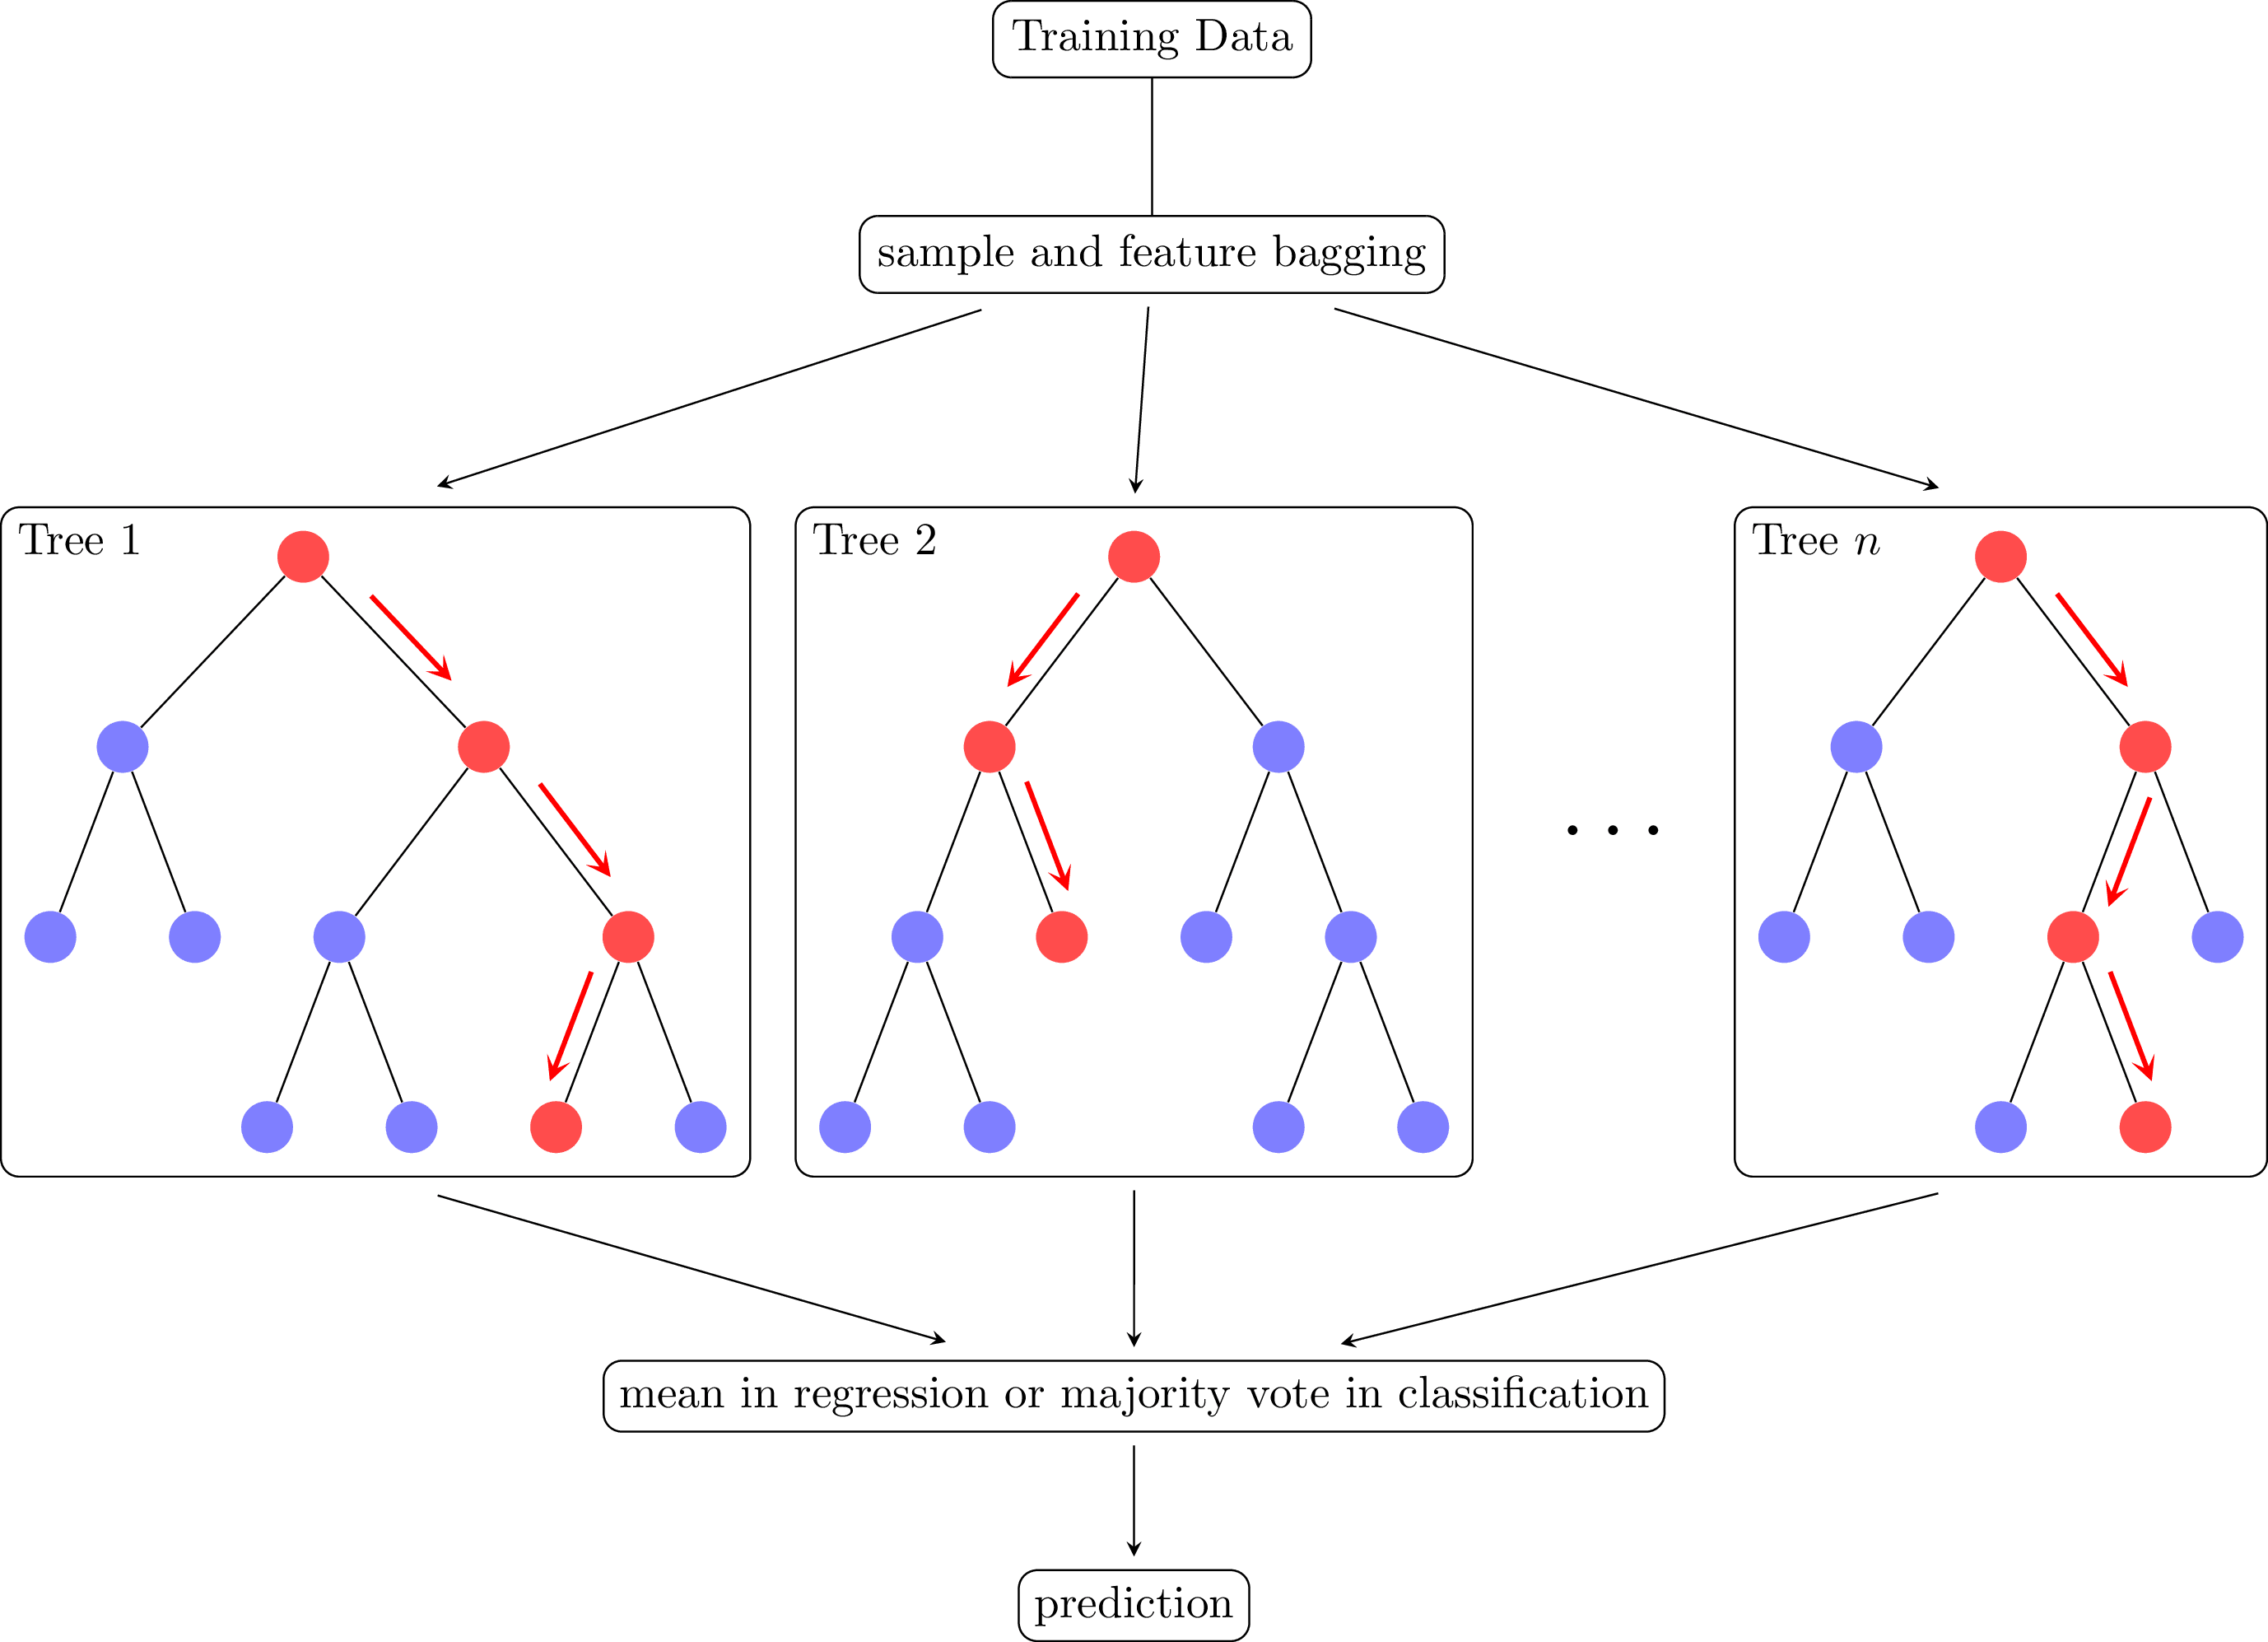
\includegraphics[width=0.88\linewidth]{Chap1/images/random-forest.png}
    \caption{Sch\'ema d'une for\^et al\'eatoire (bagging d'arbres de d\'ecision avec sous-\'echantillonnage des observations et des variables). Source : adapt\'e de~\cite{janosh2024randomforest}.}
    \label{fig:random-forest-schema}
\end{figure}
Chaque arbre voit un sous-jeu de donn\'ees diff\'erent et ne retient qu'une fraction des variables \`a chaque scission, ce qui diversifie les pr\'edictions avant leur agr\'egation finale.

\mySubSubSection{Boosting}{}
\label{sec:boosting}

Le \textbf{boosting} construit le mod\`ele de fa\c{c}on \textbf{s\'equentielle} : chaque nouvel apprenant cible les erreurs laiss\'ees par l'ensemble des apprenants pr\'ec\'edents, au lieu d'entra\^iner des mod\`eles ind\'ependants comme en bagging.
La figure~\ref{fig:boosting-schema} r\'esume cette logique additive : le mod\`ele courant est enrichi \`a chaque it\'eration par un arbre entra\^in\'e sur les r\'esidus.

\begin{figure}[H]
    \centering
    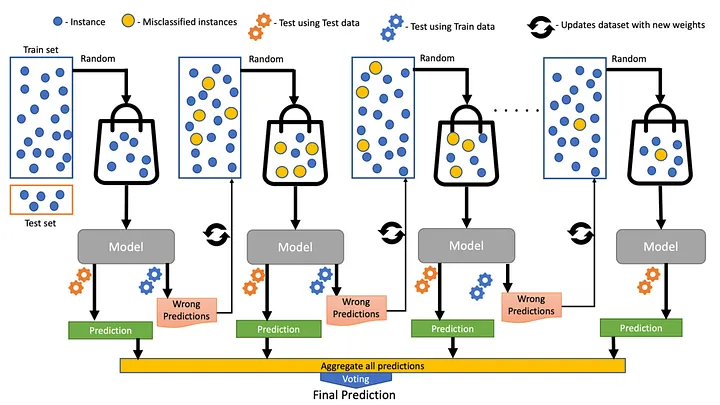
\includegraphics[width=0.82\linewidth]{Chap1/images/boosting.png}
    \caption{Principe du boosting : ajout s\'equentiel d'arbres pour corriger les erreurs du mod\`ele courant. Source : illustration p\'edagogique adapt\'ee de~\cite{verma2020xgboostillustration}.}
    \label{fig:boosting-schema}
\end{figure}
Il ressort de cette repr\'esentation que les pr\'edictions s'am\'eliorent progressivement en cumulant de petits correctifs, plut\^ot qu'en moyennant des mod\`eles parall\`eles ind\'ependants comme en bagging.

Le \textbf{gradient boosting}~\cite{friedman2001gbm} met cette id\'ee en \oe uvre en ajoutant, \`a chaque it\'eration, un arbre qui corrige les r\'esidus selon le gradient d'une fonction de perte diff\'erentiable.
On \'ecrit souvent la pr\'ediction additive sous la forme
\begin{equation}
    F_M(\mathbf{x}) = F_{M-1}(\mathbf{x}) + \eta \, h_M(\mathbf{x}),
    \label{eq:boosting}
\end{equation}
o\`u $h_M$ est un nouvel arbre entra\^in\'e sur les r\'esidus et $\eta$ un taux d'apprentissage.
Dans la pratique, le boosting construit souvent des arbres \textbf{courts} (faible profondeur) afin de corriger progressivement les erreurs sans sur-ajuster le bruit.
Le param\`etre $\eta$ (\emph{learning rate}) contr\^ole la contribution de chaque nouvel arbre : une valeur faible stabilise l'apprentissage mais exige davantage d'it\'erations.
Le nombre d'arbres, la profondeur maximale et les contraintes de r\'egularisation gouvernent ainsi le compromis entre \textbf{capacit\'e de mod\'elisation} et \textbf{g\'en\'eralisation}.

\textbf{Exemple (XGBoost et LightGBM).}
\textbf{XGBoost} (\emph{eXtreme Gradient Boosting})~\cite{chen2016xgboost} est l'une des impl\'ementations les plus utilis\'ees sur \textbf{donn\'ees tabulaires}, notamment lorsque l'on recherche un mod\`ele performant et robuste.
Son apprentissage optimise une fonction objectif compos\'ee d'un terme de perte et d'un terme de complexit\'e :
\[
\mathcal{J}^{(t)} = \sum_{i=1}^{n} l\!\left(y_i,\hat{y}_i^{(t-1)} + f_t(\mathbf{x}_i)\right) + \Omega(f_t),
\]
avec une r\'egularisation typique
\[
\Omega(f) = \gamma T + \frac{\lambda}{2}\sum_{j=1}^{T} w_j^2 + \alpha \sum_{j=1}^{T} |w_j|,
\]
o\`u $T$ est le nombre de feuilles, $w_j$ les poids des feuilles, et $(\alpha,\lambda,\gamma)$ les coefficients de p\'enalisation.
Cette formulation explicite permet de limiter la complexit\'e des arbres et de r\'eduire le surapprentissage.

En pratique, les hyperparam\`etres les plus influents sont :
\begin{itemize}
    \item \texttt{n\_estimators} : nombre d'arbres ajout\'es ;
    \item \texttt{max\_depth} : profondeur maximale des arbres ;
    \item \texttt{learning\_rate} : poids de chaque nouvel arbre ;
    \item \texttt{subsample} et \texttt{colsample\_bytree} : sous-\'echantillonnage des observations et des variables ;
    \item \texttt{reg\_alpha}, \texttt{reg\_lambda} et \texttt{gamma} : contr\^ole de la r\'egularisation.
\end{itemize}
XGBoost prend aussi en charge les valeurs manquantes en apprenant une direction de branche par d\'efaut lors des splits, et propose des impl\'ementations efficaces (\emph{histogram-based}, parall\'elisation) adapt\'ees aux volumes de donn\'ees importants.
Dans un cadre appliqu\'e, XGBoost est souvent mobilis\'e comme mod\`ele de r\'ef\'erence fort ou comme composant d'un empilement, car il combine bonne pr\'ecision, robustesse et interpr\'etabilit\'e globale (importance des variables, SHAP).

\textbf{LightGBM} (\emph{Light Gradient Boosting Machine})~\cite{ke2017lightgbm} privil\'egie une croissance des arbres \textbf{feuille par feuille} (\emph{leaf-wise}) et introduit des m\'ecanismes d'\'echantillonnage (GOSS) et de regroupement de variables (EFB) pour acc\'el\'erer l'entra\^inement sur de grands jeux de donn\'ees.




\mySubSubSection{Stacking}{}
\label{sec:stacking}

Le \textbf{stacking} (\emph{stacked generalization}) place un \textbf{m\'eta-classifieur} (ou m\'eta r\'egresseur) au-dessus de plusieurs \textbf{mod\`eles de base} de natures \'eventuellement diff\'erentes.
Chaque mod\`ele de base produit une pr\'ediction (ou une probabilit\'e) ; le m\'eta-mod\`ele apprend \`a les combiner de mani\`ere optimale, au lieu de se limiter \`a un vote fixe comme en bagging.
L'id\'ee centrale est que des mod\`eles diff\'erents capturent des \textbf{signaux compl\'ementaires} : un mod\`ele peut mieux exploiter les interactions non lin\'eaires tabulaires, un autre la structure relationnelle, un autre encore des effets locaux.
Le stacking apprend donc une \textbf{fonction de fusion} des sorties de base plut\^ot qu'une r\`egle de combinaison fix\'ee a priori.

Si l'on note $p_k(\mathbf{x})$ la sortie du $k$-i\`eme mod\`ele de base, le m\'eta-mod\`ele apprend une fonction
\[
\hat{y} = g\!\big(p_1(\mathbf{x}), p_2(\mathbf{x}), \dots, p_K(\mathbf{x})\big),
\]
o\`u $g$ peut \^etre, selon les cas, une r\'egression logistique, un arbre de d\'ecision, un gradient boosting ou un autre classifieur.
En pratique, les entr\'ees de $g$ peuvent \^etre enrichies par des variables de confiance (entropie des probabilit\'es, \'ecart entre mod\`eles, etc.).

\textbf{Exemple (m\'eta-classifieur sur sorties de bases).}
On peut par exemple empiler une for\^et al\'eatoire, un gradient boosting et un mod\`ele produisant des embeddings (graphe ou autre), puis entra\^iner un classifieur final sur les vecteurs de pr\'edictions produits par ces bases.

La figure~\ref{fig:stacking} r\'esume l'architecture hi\'erarchique du stacking.

\begin{figure}[H]
    \centering
    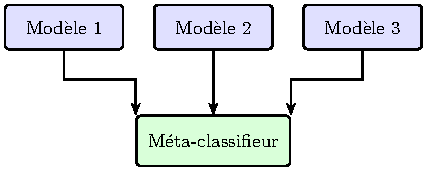
\includegraphics[width=0.78\linewidth]{Chap1/images/fig-stacking-ensemble.pdf}
    \caption{Principe du stacking : plusieurs mod\`eles de base alimentent un m\'eta-classifieur.}
    \label{fig:stacking}
\end{figure}
La figure souligne que le m\'eta-mod\`ele ne re\c{c}oit pas les variables brutes mais les sorties des apprenants de base, permettant ainsi de combiner des mod\`eles de natures diff\'erentes.

Pour \'eviter le surapprentissage, les entr\'ees du m\'eta-classifieur doivent provenir de \textbf{pr\'edictions hors \'echantillon} : les mod\`eles de base ne doivent pas avoir vu les exemples utilis\'es pour entra\^iner le m\'eta-mod\`ele.
La proc\'edure usuelle repose sur une validation crois\'ee en deux niveaux :
\begin{itemize}
    \item niveau 1 : g\'en\'erer, pour chaque observation d'entra\^inement, des pr\'edictions hors pli des mod\`eles de base ;
    \item niveau 2 : entra\^iner le m\'eta-mod\`ele sur cette matrice de m\'eta-caract\'eristiques, puis r\'eentra\^iner les mod\`eles de base sur l'ensemble d'entra\^inement.
\end{itemize}
Cette discipline m\'ethodologique est essentielle pour obtenir un gain r\'eel au test.

Le stacking est particuli\`erement utile quand la performance individuelle des mod\`eles est proche mais que leurs erreurs ne se recouvrent pas totalement.
Il peut toutefois \^etre sensible \`a la complexit\'e du m\'eta-mod\`ele et \`a la qualit\'e des pr\'edictions de base ; un protocole d'\'evaluation rigoureux reste donc indispensable.

Le tableau~\ref{tab:ensemble-comparaison} pr\'esente les trois familles d'ensembles et un exemple repr\'esentatif pour chacune ; pour les donn\'ees tabulaires de taille mod\'er\'ee, les ensembles d'arbres restent souvent tr\`es comp\'etitifs face \`a des r\'eseaux profonds g\'en\'eriques~\cite{borisov2024tabular}.

\begin{table}[h!]
    \centering
    \caption{Synth\`ese des trois familles d'ensembles et d'un exemple repr\'esentatif pour chacune.}
    \label{tab:ensemble-comparaison}
    \begin{tabular}{lp{3.2cm}p{3.2cm}p{3.5cm}}
        \hline
        Famille & Construction & Effet vis\'e & Exemple \\
        \hline
        Bagging & Parall\`ele sur tirages bootstrap & R\'eduit la variance & For\^et al\'eatoire \\
        Boosting & S\'equentielle sur les r\'esidus & R\'eduit le biais & XGBoost, LightGBM \\
        Stacking & M\'eta-mod\`ele sur les sorties des bases & Combine des mod\`eles h\'et\'erog\`enes & M\'eta-classifieur \\
        \hline
    \end{tabular}
\end{table}



\mySection{Graphes et r\'eseaux de neurones sur graphes}{}
\label{sec:graphes-gnn}

Les donn\'ees de surveillance des eaux souterraines sont souvent stock\'ees sous forme \textbf{tabulaire} (une ligne par puits, une colonne par variable).
Or, un site de pr\'el\`evement n'est pas isol\'e : il partage un contexte g\'eologique, une proximit\'e d'installations, des co-contaminants et une position g\'eographique avec d'autres sites.
Les \textbf{graphes} offrent un langage naturel pour repr\'esenter ces d\'ependances et les exploiter par apprentissage profond, en compl\'ement des mod\`eles tabulaires (for\^ets al\'eatoires, XGBoost) pr\'esent\'es en section~\ref{sec:bagging}--\ref{sec:stacking}.

\mySubSection{Repr\'esentation des donn\'ees par graphe}{}
\label{sec:graphe-basics}

Un \textbf{graphe} $G = (V, E)$ mod\'elise des entit\'es par des \textbf{n\oe uds} $v \in V$ et des liens par des \textbf{ar\^etes} $e \in E$~\cite{hamilton2017inductive}.
Chaque n\oe ud peut porter un vecteur de caract\'eristiques $\mathbf{x}_v \in \mathbb{R}^{d_v}$.
En classification de sites, on associe en g\'en\'eral \`a chaque n\oe ud \textbf{sample} (\'echantillon) une \textbf{\'etiquette} $y_v$ (par exemple contamination oui/non).

Contrairement \`a une image (grille r\'eguli\`ere) ou \`a une s\'equence (cha\^ene), un graphe autorise des connexions \textbf{irr\'eguli\`eres} : le voisinage d'un site n'est pas impos\'e par la position dans un tableau, mais par la structure relationnelle choisie.
Cette flexibilit\'e est utile lorsque l'on veut relier explicitement un puits \`a des variables de contexte (environnement, installations, qualit\'e de l'eau, regroupement g\'eographique).

On distingue :
\begin{itemize}
    \item le \textbf{graphe homog\`ene} : un seul type de n\oe ud et un seul type d'ar\^ete ;
    \item le \textbf{graphe h\'et\'erog\`ene} : plusieurs types de n\oe uds et d'ar\^etes typ\'ees, not\'ees $(s, r, t)$ pour une relation $r$ entre un n\oe ud source de type $s$ et un n\oe ud cible de type $t$.
\end{itemize}
En surveillance environnementale, l'h\'et\'erog\'en\'eit\'e refl\`ete le mod\`ele conceptuel \textbf{source, voie et r\'ecepteur} (section~\ref{sec:pfas-svr}) : sources d'activit\'e, milieux de transport, sites de mesure.


\mySubSection{R\'eseaux de neurones sur graphes}{}
\label{sec:gnn}

Les \textbf{r\'eseaux de neurones sur graphes} (GNN, \emph{Graph Neural Networks}) apprennent une \textbf{repr\'esentation vectorielle} (\emph{embedding}) pour chaque n\oe ud en diffusant l'information de proche en proche.
Le m\'ecanisme standard est le \textbf{message passing} : \`a chaque couche $\ell$, un n\oe ud agr\`ege les messages de ses voisins $\mathcal{N}(v)$ puis met \`a jour sa repr\'esentation :
\[
\mathbf{h}_v^{(\ell+1)} = \mathrm{UPDATE}\!\left(\mathbf{h}_v^{(\ell)},\, \mathrm{AGGREGATE}\big(\{\mathbf{h}_u^{(\ell)} : u \in \mathcal{N}(v)\}\big)\right).
\]

La figure~\ref{fig:message-passing} illustre ce m\'ecanisme sur un n\oe ud central et ses voisins.

\begin{figure}[H]
    \centering
    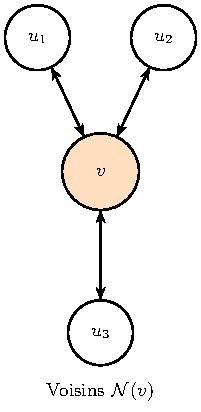
\includegraphics[width=0.55\linewidth]{Chap1/images/fig-message-passing.pdf}
    \caption{Message passing : agr\'egation des repr\'esentations des voisins $\mathcal{N}(v)$ vers le n\oe ud $v$.}
    \label{fig:message-passing}
\end{figure}
L'information locale se propage ainsi par couches successives : apr\`es $\ell$ it\'erations, $\mathbf{h}_v^{(\ell)}$ encode un voisinage \`a $\ell$ sauts~\cite{kipf2017gcn,fey2019pyg}.

Des variantes historiques incluent les \textbf{GCN} (\emph{Graph Convolutional Networks}), les \textbf{GAT} (\emph{Graph Attention Networks}) et \textbf{GraphSAGE}, qui diff\`erent par la fonction d'agr\'egation et la pond\'eration des voisins.
En pratique, ces mod\`eles sont souvent impl\'ement\'es avec des biblioth\`eques sp\'ecialis\'ees telles que \textbf{PyTorch Geometric} (PyG), qui fournit des structures de donn\'ees et des couches convolutives sur graphe~\cite{fey2019pyg}.


\mySubSection{Graphes h\'et\'erog\`enes}{}
\label{sec:graphes-heterogenes}

Un \textbf{graphe h\'et\'erog\`ene} (ou \emph{graphe typ\'e}) \'etend la d\'efinition \'el\'ementaire $G=(V,E)$ en associant un type \`a chaque n\oe ud et \`a chaque ar\^ete~\cite{hu2020hgt} :
\[
G = (V,\, E,\, \tau,\, \phi),
\]
o\`u $\tau : V \to \mathcal{T}$ est la fonction de typage des n\oe uds ($|\mathcal{T}| \geq 2$) et $\phi : E \to \mathcal{R}$ celle des ar\^etes ($|\mathcal{R}| \geq 2$).
Chaque type de n\oe ud $A \in \mathcal{T}$ dispose de son propre espace de caract\'eristiques $\mathbb{R}^{d_A}$, ce qui autorise des entit\'es de natures radicalement diff\'erentes (auteurs, articles, lieux de publication, th\`emes de recherche) \`a cohabiter dans la m\^eme structure relationnelle.

Une \textbf{m\'eta-relation} est un triplet $\langle A, r, B \rangle \in \mathcal{T} \times \mathcal{R} \times \mathcal{T}$ d\'ecrivant un lien de type $r$ entre un n\oe ud source de type $A$ et un n\oe ud cible de type $B$.
Deux n\oe uds peuvent ainsi \^etre reli\'es par des ar\^etes de s\'emantiques distinctes (co-autorat, citation, appartenance \`a un m\^eme domaine) ; le mod\`ele peut apprendre des param\`etres d'agr\'egation distincts pour chaque m\'eta-relation plut\^ot qu'un seul ensemble de param\`etres partag\'e.

Une \textbf{m\'eta-chemin} d\'esigne une s\'equence ordonn\'ee de types de n\oe uds reli\'es par des types de relations :
\[
\mathcal{P} :\ A_0 \xrightarrow{r_1} A_1 \xrightarrow{r_2} A_2 \;\cdots\; \xrightarrow{r_\ell} A_\ell.
\]
Les m\'eta-chemins capturent des d\'ependances s\'emantiques compos\'ees qui ne sont pas visibles dans le voisinage imm\'ediat.
Par exemple, dans un r\'eseau acad\'emique, le m\'eta-chemin $\texttt{Auteur} \xrightarrow{\text{\'ecrit}} \texttt{Article} \xrightarrow{\text{\'ecrit\_par}} \texttt{Auteur}$ identifie deux chercheurs ayant co-publi\'e sans qu'une ar\^ete directe entre eux soit pr\'esente dans le graphe.

Ce formalisme s'applique dans de nombreux domaines o\`u les entit\'es et leurs relations sont intrins\`equement h\'et\'erog\`enes : r\'eseaux acad\'emiques (auteurs, articles, lieux, domaines)~\cite{hu2020hgt}, graphes biom\'edicaux associant g\`enes, maladies et m\'edicaments, graphes de connaissance \`a large \'echelle, ou encore r\'eseaux de surveillance environnementale o\`u plusieurs cat\'egories d'entit\'es sont reli\'ees par des liens typ\'es.
La conception du graphe h\'et\'erog\`ene utilis\'e dans cette \'etude est d\'etaill\'ee au chapitre~3.

Contrairement aux GNN homog\`enes, les GNN h\'et\'erog\`enes doivent g\'erer simultan\'ement des espaces de caract\'eristiques de dimensions diff\'erentes selon le type de n\oe ud.
La solution usuelle est de projeter les vecteurs de chaque type dans un espace latent commun de dimension $d$ avant les op\'erations d'agr\'egation, puis de sp\'ecialiser les param\`etres d'attention selon la m\'eta-relation.
C'est pr\'ecis\'ement ce m\'ecanisme que le \textbf{HGT} (section~\ref{sec:hgt}) formalise par des matrices de cl\'e ($\mathbf{K}$), de requ\^ete ($\mathbf{Q}$) et de valeur ($\mathbf{V}$) propres \`a chaque type de n\oe ud et de relation.


\mySubSection{Heterogeneous Graph Transformer (HGT)}{}
\label{sec:hgt}

Le \textbf{Heterogeneous Graph Transformer} (HGT)~\cite{hu2020hgt} adapte le m\'ecanisme d'\textbf{attention} des transformeurs aux graphes h\'et\'erog\`enes.
Pour une m\'eta-relation $(\tau_s, \phi, \tau_t)$, les poids d'attention d\'ependent du type de n\oe ud source, du type de relation et du type de n\oe ud cible.
Chaque type dispose de projections sp\'ecifiques (matrices requ\^ete, cl\'e, valeur), ce qui permet d'apprendre des interactions diff\'erenci\'ees entre, par exemple, un lien \emph{g\'eographique} et un lien \emph{de qualit\'e de l'eau}.

Pour un message envoy\'e d'un voisin $u$ vers un n\oe ud cible $v$, l'attention peut s'\'ecrire sch\'ematiquement :
\[
\alpha_{uv} = \mathrm{softmax}\!\left(\frac{(\mathbf{K}_{\tau(u)}\,\mathbf{h}_u)^{\top}(\mathbf{Q}_{\tau(v)}\,\mathbf{h}_v)}{\sqrt{d}}\right),
\qquad
\mathbf{h}_v' = \sum_{u \in \mathcal{N}(v)} \alpha_{uv}\, \mathbf{V}_{\phi(u,v)} \mathbf{h}_u,
\]
o\`u $\mathbf{K}_{\tau(u)}$ (cl\'e, type source) et $\mathbf{Q}_{\tau(v)}$ (requ\^ete, type cible) sont des projections sp\'ecifiques au type, et $\mathbf{V}$ d\'epend du type de relation~\cite{hu2020hgt}.
Des couches \texttt{HGTConv} sont empil\'ees pour produire, en sortie, un \textbf{embedding} de dimension fixe pour chaque n\oe ud \texttt{sample}.

La figure~\ref{fig:hgt-architecture} illustre le m\'ecanisme d'attention h\'et\'erog\`ene du HGT : les n\oe uds sources projettent leurs repr\'esentations via les matrices cl\'e ($\mathbf{K}$), les n\oe uds cibles via les matrices requ\^ete ($\mathbf{Q}$), et les valeurs ($\mathbf{V}$) sont pond\'er\'ees par les scores d'attention avant agr\'egation.

\begin{figure}[htbp]
    \centering
    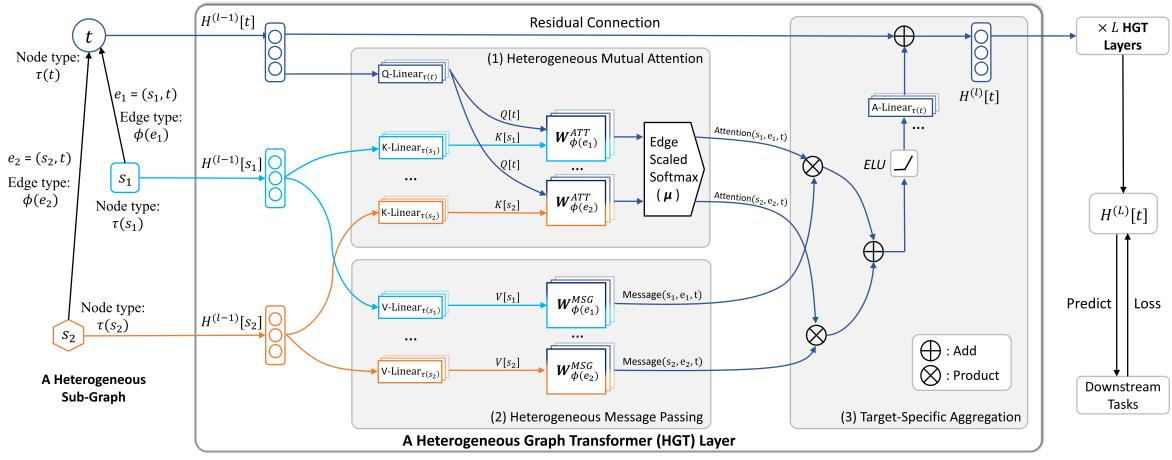
\includegraphics[width=0.90\linewidth]{Chap1/images/HGT.png}
    \caption{Architecture du Heterogeneous Graph Transformer (HGT) : attention typ\'ee par m\'eta-relation pour la propagation de l'information dans un graphe h\'et\'erog\`ene. Source : adapt\'e de~\cite{hu2020hgt}.}
    \label{fig:hgt-architecture}
\end{figure}
La figure souligne que chaque m\'eta-relation $(\tau_s, \phi, \tau_t)$ dispose de ses propres param\`etres de projection, ce qui permet au mod\`ele d'apprendre des interactions s\'emantiquement diff\'erentes selon la nature des n\oe uds et des liens connect\'es.

Cet embedding r\'esume l'information relationnelle diffus\'ee dans le graphe (contexte environnemental, proximit\'e d'installations, co-contaminants, voisinage g\'eographique).
Il peut ensuite \^etre exploit\'e de deux mani\`eres compl\'ementaires, au coeur des approches hybrides :
\begin{itemize}
    \item \textbf{Fusion par embeddings} : concat\'enation des embeddings HGT avec les variables tabulaires d'origine, puis apprentissage d'un classifieur XGBoost sur l'espace enrichi ;
    \item \textbf{Stacking} : utilisation des probabilit\'es ou embeddings HGT comme entr\'ees d'un m\'eta-classifieur, aux c\^ot\'es d'autres mod\`eles tabulaires (section~\ref{sec:stacking}).
\end{itemize}
Cette dualit\'e r\'ev\`ele un pont entre \textbf{donn\'ees relationnelles} (graphe) et \textbf{mod\`eles tabulaires} (boosting), utile lorsque la structure spatiale et contextuelle apporte un signal que les seules colonnes isol\'ees ne capturent pas enti\`erement.


\mySection{Interpr\'etabilit\'e des mod\`eles}{}
\label{sec:interpretabilite}

Un mod\`ele pr\'ecis mais opaque limite l'acceptation par les gestionnaires de l'eau et les r\'egulateurs : une d\'ecision de contr\^ole, de priorisation de campagnes ou de fermeture de puits exige une \textbf{justification} compr\'ehensible et reproductible.
En sant\'e environnementale, l'interpr\'etabilit\'e n'est plus un simple compl\'ement esth\'etique : elle conditionne la confiance des parties prenantes et la possibilit\'e de confronter les sorties algorithmiques \`a des connaissances de terrain (hydrog\'eologie, usages industriels, co-contaminants).
Cette section pr\'esente les notions n\'ecessaires pour lire les analyses men\'ees dans la contribution, en particulier l'approche \textbf{SHAP} et son d\'eploiement sur les mod\`eles tabulaires, fusionn\'es et empil\'es d\'ecrits aux sections~\ref{sec:stacking} et~\ref{sec:hgt}.


\mySubSection{Enjeux et interpr\'etabilit\'e a posteriori}{}
\label{sec:interpretabilite-enjeux}

On distingue en pratique deux familles d'approches.
L'interpr\'etabilit\'e \textbf{intrins\`eque} repose sur des mod\`eles structurellement lisibles (arbres de d\'ecision peu profonds, r\'egressions lin\'eaires avec coefficients explicites).
L'interpr\'etabilit\'e \textbf{a posteriori} (\emph{post-hoc}) applique, apr\`es entra\^inement, des m\'ethodes qui expliquent les pr\'edictions d'un mod\`ele potentiellement complexe (for\^et al\'eatoire, gradient boosting, r\'eseau sur graphe).
Les importances par impuret\'e des for\^ets al\'eatoires (section~\ref{sec:bagging}) donnent un ordre de grandeur global, mais elles ne d\'ecrivent pas la contribution \`a une pr\'ediction individuelle ni ne satisfont des axiomes de r\'epartition \'equitable entre variables corr\'el\'ees.
Les importances par permutation~\cite{breiman2001rf} corrigent partiellement ce biais en mesurant la d\'egradation de performance lorsqu'une variable est m\'elang\'ee al\'eatoirement sur l'\'echantillon de validation ; elles s'appliquent \`a tout type de mod\`ele mais restent globales, insensibles \`a la direction de l'effet et co\^uteuses \`a calculer quand le nombre de variables est \'elev\'e.

\textbf{LIME} (\emph{Local Interpretable Model-agnostic Explanations})~\cite{ribeiro2016lime} adopte une logique locale : pour chaque observation, un mod\`ele lin\'eaire interpr\'etable est ajust\'e sur des perturbations de l'entr\'ee pond\'er\'ees par leur proximit\'e au point d'int\'er\^et.
La flexibilit\'e de LIME est un atout, mais la stabilit\'e des explications d\'epend fortement du protocole d'\'echantillonnage et peut varier d'une ex\'ecution \`a l'autre, ce qui limite son usage dans des contextes r\'eglementaires exigeant la reproductibilit\'e.

L'approche \textbf{SHAP} (\emph{SHapley Additive exPlanations})~\cite{lundberg2017shap} fournit un cadre unifi\'e : chaque variable re\c{c}oit une contribution additive \`a la pr\'ediction, fond\'ee sur la th\'eorie des jeux coop\'eratifs.
Elle s'applique naturellement aux mod\`eles \`a arbres mobilis\'es dans ce m\'emoire (XGBoost, LightGBM) via l'algorithme \textbf{TreeSHAP}, et se prolonge aux espaces de features enrichis (fusion d'embeddings, m\'eta-caract\'eristiques de stacking).


\mySubSection{Valeurs de Shapley et d\'ecomposition additive}{}
\label{sec:shapley-shap}

Pour une pr\'ediction $f(\mathbf{x})$ sur un vecteur de variables $\mathbf{x} = (x_1,\ldots,x_p)$, la contribution SHAP de la variable $i$ repose sur la \textbf{valeur de Shapley} :
\begin{equation}
    \phi_i = \sum_{S \subseteq \mathcal{F} \setminus \{i\}}
    \frac{|S|!\,(|\mathcal{F}|-|S|-1)!}{|\mathcal{F}|!}
    \bigl[f(S \cup \{i\}) - f(S)\bigr],
    \label{eq:shapley}
\end{equation}
o\`u $\mathcal{F} = \{1,\ldots,p\}$ est l'ensemble des indices de variables et $f(S)$ la pr\'ediction moyenne du mod\`ele lorsque seules les variables de la coalition $S$ sont observ\'ees, les autres \'etant marginalis\'ees selon la distribution de r\'ef\'erence (souvent l'\'echantillon d'entra\^inement ou de test).

Chaque variable est vue comme un \emph{joueur} ; la coalition $S$ repr\'esente un sous-ensemble de variables disponibles pour la pr\'ediction.
Le terme $f(S \cup \{i\}) - f(S)$ mesure le \textbf{gain marginal} de $i$ lorsque $S$ est d\'ej\`a connu ; la formule~\eqref{eq:shapley} en fait la moyenne pond\'er\'ee sur toutes les coalitions, ce qui \'evite qu'une variable corr\'el\'ee monopolise tout le cr\'edit ou soit ignor\'ee selon l'ordre d'introduction.

Cette construction v\'erifie des propri\'et\'es souhaitables~\cite{lundberg2017shap} :
\begin{itemize}
    \item \textbf{Efficacit\'e} : $\sum_{i=1}^{p} \phi_i = f(\mathbf{x}) - \mathbb{E}[f(\mathbf{X})]$, o\`u $\mathbb{E}[f(\mathbf{X})]$ est la \textbf{valeur de base} (\emph{expected value}) du mod\`ele ;
    \item \textbf{Sym\'etrie} : deux variables ayant la m\^eme contribution marginale sur toute coalition re\c{c}oivent la m\^eme valeur SHAP ;
    \item \textbf{Nullit\'e} : une variable sans effet re\c{c}oit $\phi_i = 0$ ;
    \item \textbf{Additivit\'e} : pour un ensemble de mod\`eles combin\'es additivement, les contributions se somment.
\end{itemize}

La pr\'ediction s'\'ecrit ainsi sous forme additive :
\[
f(\mathbf{x}) = \phi_0 + \sum_{i=1}^{p} \phi_i,
\qquad
\phi_0 = \mathbb{E}[f(\mathbf{X})],
\]
ce qui permet de lire, pour chaque observation, quelles variables \textbf{augmentent} ou \textbf{diminuent} la sortie du mod\`ele par rapport \`a la moyenne.

Le calcul exact de l'\'equation~\eqref{eq:shapley} est exponentiel en $p$ (toutes les coalitions).
\textbf{TreeSHAP}~\cite{lundberg2017shap} exploite la structure des arbres de d\'ecision pour obtenir des valeurs SHAP \textbf{exactes} en temps polynomial pour XGBoost, LightGBM et les for\^ets al\'eatoires.
En pratique, on instancie un \texttt{TreeExplainer} sur le booster entra\^in\'e ; \`a d\'efaut, XGBoost expose aussi des \emph{pred\_contribs} (contributions par feuille) compatibles avec la m\^eme lecture additive.


\mySubSection{Analyses globale et locale}{}
\label{sec:shap-global-local}

Les sorties SHAP se lisent \`a deux \'echelles compl\'ementaires.

\paragraph{Niveau global.}
On agr\`ege typiquement les valeurs absolues $|\phi_i|$ sur un jeu d'observations (souvent l'\'echantillon de test) pour obtenir une \textbf{importance moyenne} par variable.
Le graphique en barres (\emph{bar plot}) classe les variables par ordre d\'ecroissant de cette importance.
Le graphique en nuage (\emph{beeswarm}, ou \emph{summary plot}) repr\'esente, pour chaque variable, la distribution des $\phi_i$ : la position horizontale indique l'ampleur et le signe de l'effet, la couleur le niveau de la variable (faible ou \'elev\'e).
On observe ainsi non seulement \emph{quelles} variables comptent le plus, mais aussi si une valeur \'elev\'ee de la variable pousse g\'en\'eralement vers la classe positive ou n\'egative~\cite{lundberg2017shap}.

\paragraph{Niveau local.}
Pour une observation $\mathbf{x}^{(j)}$ (un puits, un point de surveillance), les $\phi_i^{(j)}$ d\'ecrivent la pr\'ediction individuelle.
Le \textbf{graphique de force} (\emph{force plot}) aligne les contributions positives (vers la classe \emph{contamin\'e}) et n\'egatives (vers la classe \emph{non contamin\'e}) autour de la valeur de base $\phi_0$.
Un barplot local des $| \phi_i^{(j)} |$ les plus \'elev\'es offre une vue synth\'etique pour un cas d'\'etude.
Ces vues sont utiles pour expliquer \`a un expert pourquoi un site pr\'ecis a \'et\'e class\'e \`a risque, au-del\`a d'un score global.

\paragraph{Relations non lin\'eaires.}
Les \textbf{graphiques de d\'ependance} (\emph{dependence plots}) repr\'esentent, pour une variable $i$, la valeur de $x_i$ en abscisse et $\phi_i$ en ordonn\'ee.
Ils mettent en \'evidence des effets \`a seuil, des saturations ou des interactions (en colorant les points selon une deuxi\`eme variable corr\'el\'ee).
Pour des classifieurs par arbres, on peut y v\'erifier que le mod\`ele reproduit des comportements plausibles (par exemple une influence accrue de la proximit\'e d'une source industrielle au-del\`a d'un certain rayon), sans confondre cette coh\'erence avec une preuve causale.


\mySubSection{Limites et recul \'epist\'emologique}{}
\label{sec:interpretabilite-limites}

Une variable importante au sens SHAP (proximit\'e d'une installation, co-contaminant, embedding li\'e \`a un cluster g\'eographique) signale une \textbf{association statistique} apprise par le mod\`ele, pas un m\'ecanisme physique d\'emonstr\'e.
Les variables corr\'el\'ees se partagent le cr\'edit : l'ordre d'importance peut varier selon l'\'echantillon et la distribution de r\'ef\'erence.
Les explications portent sur le \textbf{mod\`ele entra\^in\'e} et le jeu de donn\'ees consid\'er\'e ; un r\'eentra\^inement ou un changement de protocole (par exemple passage au mode confirmatoire avec concentrations PFAS) peut modifier les profils SHAP m\^eme si les tendances physiques demeurent qualitatives.

Pour le HGT, la partie du signal port\'ee par la \textbf{topologie} du graphe (chemins entre \texttt{facility}, \texttt{env}, \texttt{sample}) n'est pas enti\`erement d\'epli\'ee dans les graphiques tabulaires ou d'embeddings.
Enfin, l'usage op\'erationnel suppose une \textbf{lecture conjointe} avec des hydrog\'eologues et des toxicologues : l'outil priorise et explique, la d\'ecision publique reste argument\'ee au-del\`a du seul score algorithmique.


\mySection{Synth\`ese}{}
\label{sec:synthese-chap1}

Ce chapitre a introduit, de mani\`ere autonome et progressive, les concepts mobilis\'es dans la suite du m\'emoire.
Les \textbf{PFAS} ont \'et\'e pr\'esent\'es comme polluants persistants, soumis \`a un encadrement r\'eglementaire de plus en plus strict.
Les paradigmes de l'\textbf{apprentissage automatique} (supervis\'e, non supervis\'e, semi-supervis\'e et par renforcement), les m\'ethodes d'ensemble par \textbf{bagging} (for\^et al\'eatoire), \textbf{boosting} (XGBoost, LightGBM) et \textbf{stacking} (m\'eta-classifieur) constituent le socle des m\'ethodes pr\'edictives en donn\'ees tabulaires.
Les \textbf{graphes h\'et\'erog\`enes}, les GNN, le \textbf{HGT} et les sch\'emas de fusion ou de stacking entre embeddings graphiques et mod\`eles tabulaires, pr\'eparent la lecture des approches hybrides d\'evelopp\'ees dans la suite du m\'emoire.
Enfin, \textbf{SHAP} et TreeSHAP (analyses globale et locale, graphiques de d\'ependance) permettent d'expliquer les mod\`eles tabulaires, la fusion embeddings--XGBoost, le stacking sur m\'eta-caract\'eristiques et, partiellement, le HGT par sensibilit\'e au gradient ; cette interpr\'etabilit\'e conditionne une utilisation responsable en sant\'e environnementale, sous r\'eserve d'un recul sur la causalit\'e.

